\section{Aho - Corasick Step by step}

\subsection{Problem}
Given the text: "DIDUDUADI".

Given the 6 patterns: "DI", "DIDU", "DIDI", "DU", "DUDUA", "DUADI".

Count how many patterns are there occur in the text?

\subsection{Main idea\cite{stanford}}
Aho-Corsick has 2 steps:

Step 1: Preprocessing process: Aho-Corasick uses trie structure to contain multiple patterns. In this trie structure, every node has a suffix link. At node i, the suffix link points to a node satisfies that prefix ends at that node is the longest suffix of string ending at node i.

Step 2: Searching/ Matching process: Aho-Corasick uses suffix link to link to the prefix when the mismatching occurs, so that we don’t have to check the same substring many times.
\subsection{Preprocessing\cite{vnoj}\cite{CpAlgor}}
There are two substeps in this process:

Step 1: Initialize a trie with suffix link pointing to the root to contain patterns.

Step 2: Linking the suffix link of each node to the node that satisfies the condition.

\subsubsection*{Initialize the trie with suffix link points to the root}
\pagebreak
\subsubsection*{Source code}
\lstinputlisting[language=C++]{code/initialize.cpp}
\subsubsection*{Result}
\begin{center}
    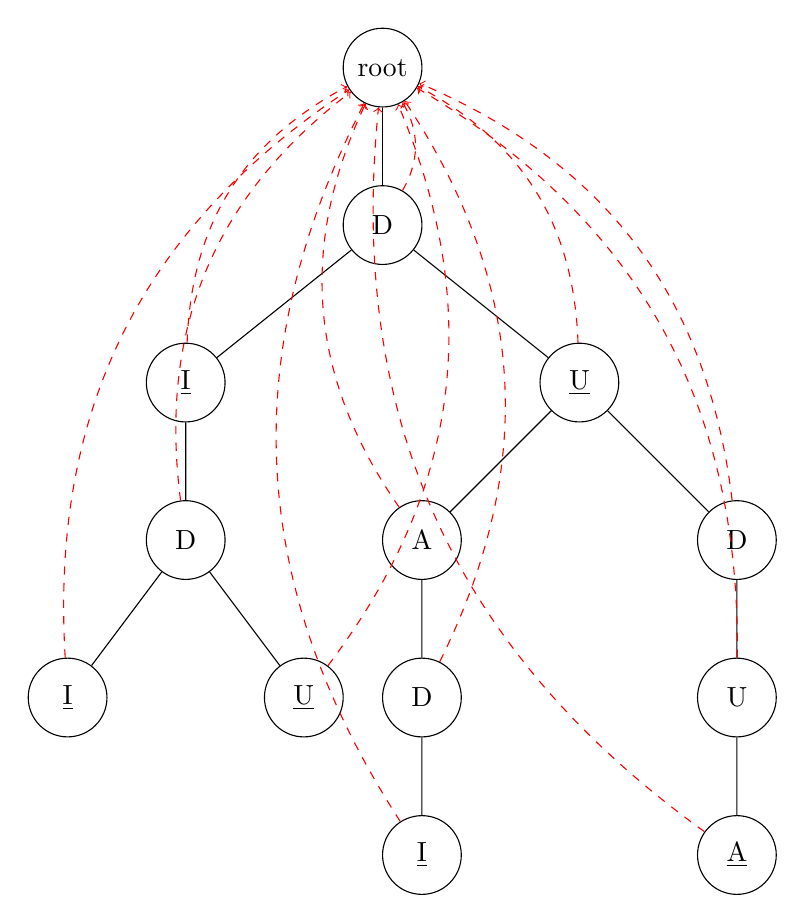
\begin{tikzpicture}[
        level 1/.style={sibling distance=6cm, level distance=2cm},
        level 2/.style={sibling distance=5cm, level distance=2cm},
        level 3/.style={sibling distance=4cm, level distance=2cm},
        level 4/.style={sibling distance=3cm, level distance=2cm},
        level 5/.style={sibling distance=2cm, level distance=2cm},
        level 6/.style={sibling distance=2cm, level distance=2ccm},
        every node/.style={circle, draw, minimum size=1cm}
    ]
        % Vẽ cây chính
        \node (root) {root}
            child { node (D1) {D}
                child { node (I) {\underline{I}}
                    child { node (D2) {D}
                        child { node (I2) {\underline{I} }}
                        child { node (U2) {\underline{U} }}
                    }
                }
                child { node (U1) {\underline{U}}
                    child { node (A2) {A}
                        child { node (D4) {D}
                            child { node (I3) {\underline{I} } }
                        }
                    }
                    child { node (D3) {D}
                        child { node (U3) {U}
                            child { node (A) {\underline{A} } }
                        }
                    }
                }
            };

        % Thêm các liên kết về gốc
        \draw[red, dashed, ->] (D1) to[bend right] (root);
        \draw[red, dashed, ->] (I) to[bend left] (root);
        \draw[red, dashed, ->] (I2) to[bend left] (root);
        \draw[red, dashed, ->] (D2) to[bend left] (root);
        \draw[red, dashed, ->] (U1) to[bend right] (root);
        \draw[red, dashed, ->] (D3) to[bend right] (root);
        \draw[red, dashed, ->] (U2) to[bend right] (root);
        \draw[red, dashed, ->] (A) to[bend left] (root);
        \draw[red, dashed, ->] (A2) to[bend left] (root);
        \draw[red, dashed, ->] (D4) to[bend right] (root);
        \draw[red, dashed, ->] (I3) to[bend left] (root);
        \draw[red, dashed, ->] (U3) to[bend right] (root);
    \end{tikzpicture}
\end{center}
\pagebreak
\subsection*{Linking the suffix link}
\subsubsection*{Source code}
\lstinputlisting[language=C++]{code/linking.cpp}
\pagebreak
\subsubsection*{Step by step}
\textbf{Step 1:}
\begin{center}
    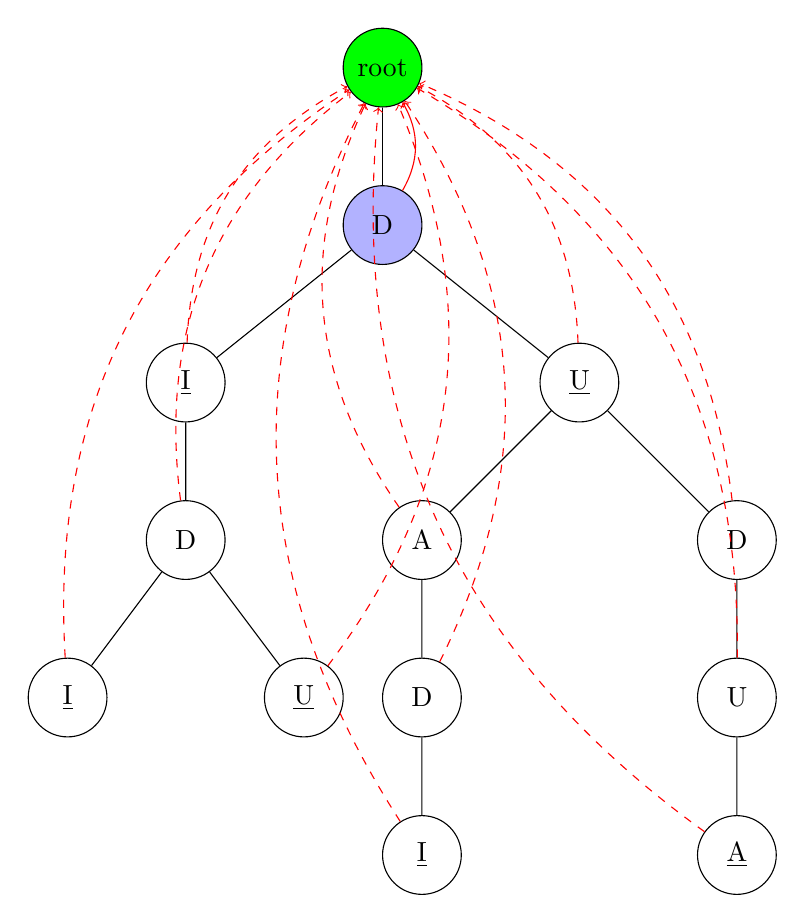
\begin{tikzpicture}[
        level 1/.style={sibling distance=6cm, level distance=2cm},
        level 2/.style={sibling distance=5cm, level distance=2cm},
        level 3/.style={sibling distance=4cm, level distance=2cm},
        level 4/.style={sibling distance=3cm, level distance=2cm},
        level 5/.style={sibling distance=2cm, level distance=2cm},
        level 6/.style={sibling distance=2cm, level distance=2ccm},
        every node/.style={circle, draw, minimum size=1cm}
    ]
        % Vẽ cây chính
        \node [fill=green](root) {root}
            child { node[fill=blue!30] (D1) {D}
                child { node (I) {\underline{I}}
                    child { node (D2) {D}
                        child { node (I2) {\underline{I}} }
                        child { node (U2) {\underline{U}} }
                    }
                }
                child { node (U1) {\underline{U}}
                    child { node (A2) {A}
                        child { node (D4) {D}
                            child { node (I3) {\underline{I}} }
                        }
                    }
                    child { node (D3) {D}
                        child { node (U3) {U}
                            child { node (A) {\underline{A}} }
                        }
                    }
                }
            };

        % Thêm các liên kết về gốc
        \draw[red, ->] (D1) to[bend right] (root);
        \draw[red, dashed, ->] (I) to[bend left] (root);
        \draw[red, dashed, ->] (I2) to[bend left] (root);
        \draw[red, dashed, ->] (D2) to[bend left] (root);
        \draw[red, dashed, ->] (U1) to[bend right] (root);
        \draw[red, dashed, ->] (D3) to[bend right] (root);
        \draw[red, dashed, ->] (U2) to[bend right] (root);
        \draw[red, dashed, ->] (A) to[bend left] (root);
        \draw[red, dashed, ->] (A2) to[bend left] (root);
        \draw[red, dashed, ->] (D4) to[bend right] (root);
        \draw[red, dashed, ->] (I3) to[bend left] (root);
        \draw[red, dashed, ->] (U3) to[bend right] (root);
    \end{tikzpicture}
\end{center}
Travel from root to node D, the parent is the root so we do nothing.
\pagebreak

\textbf{Step 2:}
\begin{center}
    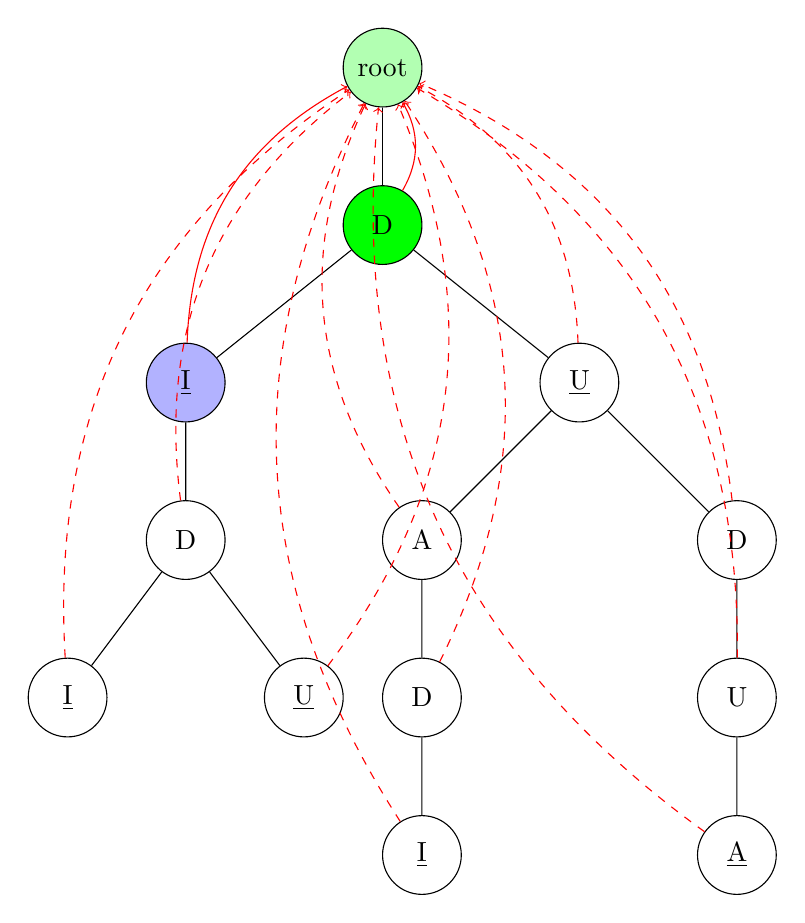
\begin{tikzpicture}[
        level 1/.style={sibling distance=6cm, level distance=2cm},
        level 2/.style={sibling distance=5cm, level distance=2cm},
        level 3/.style={sibling distance=4cm, level distance=2cm},
        level 4/.style={sibling distance=3cm, level distance=2cm},
        level 5/.style={sibling distance=2cm, level distance=2cm},
        level 6/.style={sibling distance=2cm, level distance=2ccm},
        every node/.style={circle, draw, minimum size=1cm}
    ]
        % Vẽ cây chính
        \node [fill=green!30](root) {root}
            child { node [fill=green](D1) {D}
                child { node [fill=blue!30] (I) {\underline{I}}
                    child { node (D2) {D}
                        child { node (I2) {\underline{I}} }
                        child { node (U2) {\underline{U}} }
                    }
                }
                child { node (U1) {\underline{U}}
                    child { node (A2) {A}
                        child { node (D4) {D}
                            child { node (I3) {\underline{I}} }
                        }
                    }
                    child { node (D3) {D}
                        child { node (U3) {U}
                            child { node (A) {\underline{A}} }
                        }
                    }
                }
            };

        % Thêm các liên kết về gốc
        \draw[red, ->] (D1) to[bend right] (root);
        \draw[red, ->] (I) to[bend left] (root);
        \draw[red, dashed, ->] (I2) to[bend left] (root);
        \draw[red, dashed, ->] (D2) to[bend left] (root);
        \draw[red, dashed, ->] (U1) to[bend right] (root);
        \draw[red, dashed, ->] (D3) to[bend right] (root);
        \draw[red, dashed, ->] (U2) to[bend right] (root);
        \draw[red, dashed, ->] (A) to[bend left] (root);
        \draw[red, dashed, ->] (A2) to[bend left] (root);
        \draw[red, dashed, ->] (D4) to[bend right] (root);
        \draw[red, dashed, ->] (I3) to[bend left] (root);
        \draw[red, dashed, ->] (U3) to[bend right] (root);
    \end{tikzpicture}

    Travel to node I. The parent of this node is node D. 
    
    The suffix link of node D points to the root. 
    
    The root doesn't have node I as its child so we do nothing
\end{center}
\pagebreak

\textbf{Step 3:}
\begin{center}
    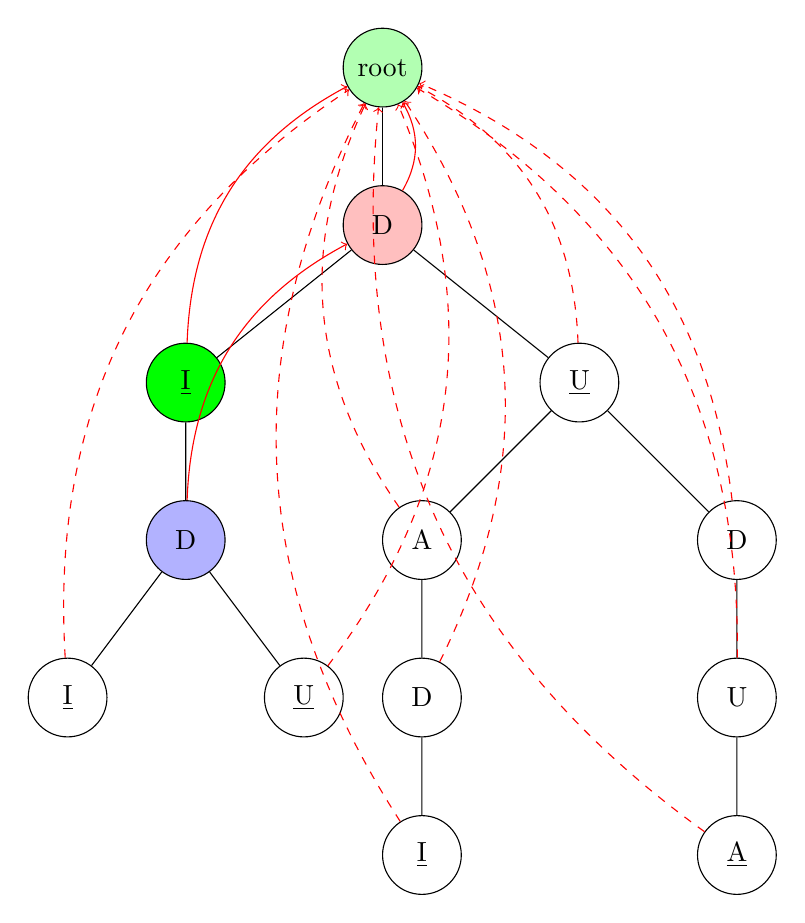
\begin{tikzpicture}[
        level 1/.style={sibling distance=6cm, level distance=2cm},
        level 2/.style={sibling distance=5cm, level distance=2cm},
        level 3/.style={sibling distance=4cm, level distance=2cm},
        level 4/.style={sibling distance=3cm, level distance=2cm},
        level 5/.style={sibling distance=2cm, level distance=2cm},
        level 6/.style={sibling distance=2cm, level distance=2ccm},
        every node/.style={circle, draw, minimum size=1cm}
    ]
        % Vẽ cây chính
        \node [fill=green!30](root) {root}
            child { node [fill=pink](D1) {D}
                child { node [fill=green] (I) {\underline{I}}
                    child { node [fill=blue!30](D2) {D}
                        child { node (I2) {\underline{I}} }
                        child { node (U2) {\underline{U}} }
                    }
                }
                child { node (U1) {\underline{U}}
                    child { node (A2) {A}
                        child { node (D4) {D}
                            child { node (I3) {\underline{I}} }
                        }
                    }
                    child { node (D3) {D}
                        child { node (U3) {U}
                            child { node (A) {\underline{A}} }
                        }
                    }
                }
            };

        % Thêm các liên kết về gốc
        \draw[red, ->] (D1) to[bend right] (root);
        \draw[red, ->] (I) to[bend left] (root);
        \draw[red, dashed, ->] (I2) to[bend left] (root);
        \draw[red, ->] (D2) to[bend left] (D1);
        \draw[red, dashed, ->] (U1) to[bend right] (root);
        \draw[red, dashed, ->] (D3) to[bend right] (root);
        \draw[red, dashed, ->] (U2) to[bend right] (root);
        \draw[red, dashed, ->] (A) to[bend left] (root);
        \draw[red, dashed, ->] (A2) to[bend left] (root);
        \draw[red, dashed, ->] (D4) to[bend right] (root);
        \draw[red, dashed, ->] (I3) to[bend left] (root);
        \draw[red, dashed, ->] (U3) to[bend right] (root);
    \end{tikzpicture}

\end{center}
Travel to node D. The parent of this node is node I. 
    
The suffix link of node I points to the root. 
    
The root has node D as its child so the suffix link is now pointing to that node.
\pagebreak

\textbf{Step 4:}
\begin{center}
    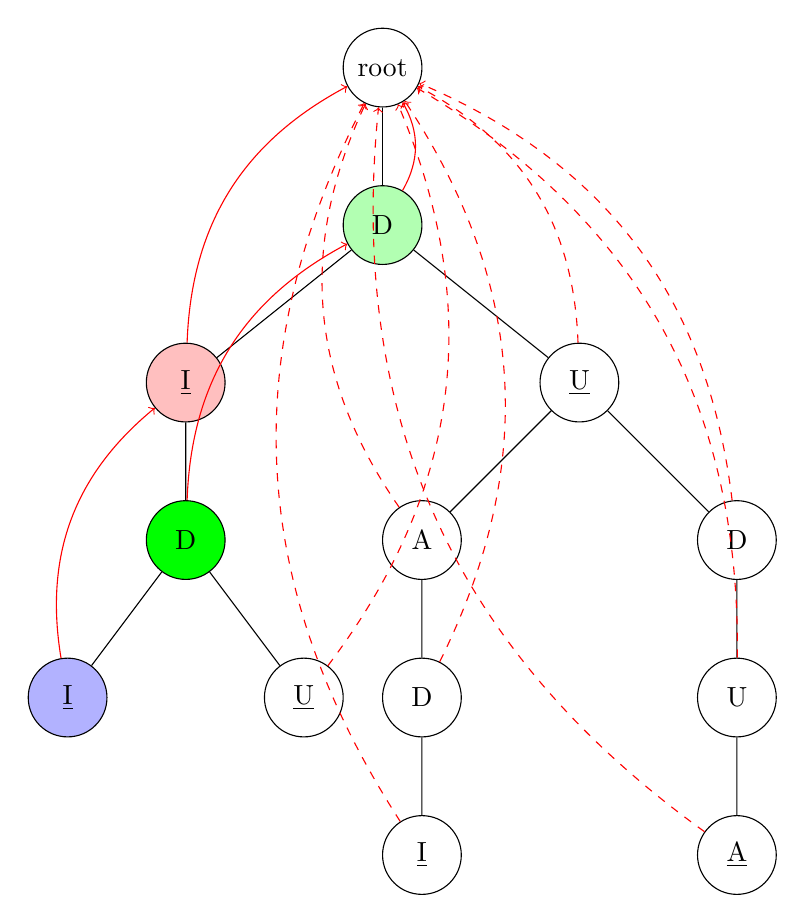
\begin{tikzpicture}[
        level 1/.style={sibling distance=6cm, level distance=2cm},
        level 2/.style={sibling distance=5cm, level distance=2cm},
        level 3/.style={sibling distance=4cm, level distance=2cm},
        level 4/.style={sibling distance=3cm, level distance=2cm},
        level 5/.style={sibling distance=2cm, level distance=2cm},
        level 6/.style={sibling distance=2cm, level distance=2ccm},
        every node/.style={circle, draw, minimum size=1cm}
    ]
        % Vẽ cây chính
        \node (root) {root}
            child { node [fill=green!30](D1) {D}
                child { node [fill=pink](I) {\underline{I}}
                    child { node [fill=green](D2) {D}
                        child { node [fill=blue!30](I2) {\underline{I}} }
                        child { node (U2) {\underline{U}} }
                    }
                }
                child { node (U1) {\underline{U}}
                    child { node (A2) {A}
                        child { node (D4) {D}
                            child { node (I3) {\underline{I}} }
                        }
                    }
                    child { node (D3) {D}
                        child { node (U3) {U}
                            child { node (A) {\underline{A}} }
                        }
                    }
                }
            };

        % Thêm các liên kết về gốc
        \draw[red, ->] (D1) to[bend right] (root);
        \draw[red, ->] (I) to[bend left] (root);
        \draw[red, ->] (I2) to[bend left] (I);
        \draw[red, ->] (D2) to[bend left] (D1);
        \draw[red, dashed, ->] (U1) to[bend right] (root);
        \draw[red, dashed, ->] (D3) to[bend right] (root);
        \draw[red, dashed, ->] (U2) to[bend right] (root);
        \draw[red, dashed, ->] (A) to[bend left] (root);
        \draw[red, dashed, ->] (A2) to[bend left] (root);
        \draw[red, dashed, ->] (D4) to[bend right] (root);
        \draw[red, dashed, ->] (I3) to[bend left] (root);
        \draw[red, dashed, ->] (U3) to[bend right] (root);
    \end{tikzpicture}

\end{center}
Travel to node I. The parent of this node is node D. 
    
The suffix link of node D points to the other node D. 
    
The other node D has node U as its child so the suffix link is now pointing to that node.
\pagebreak

\textbf{Step 5:}
\begin{center}
    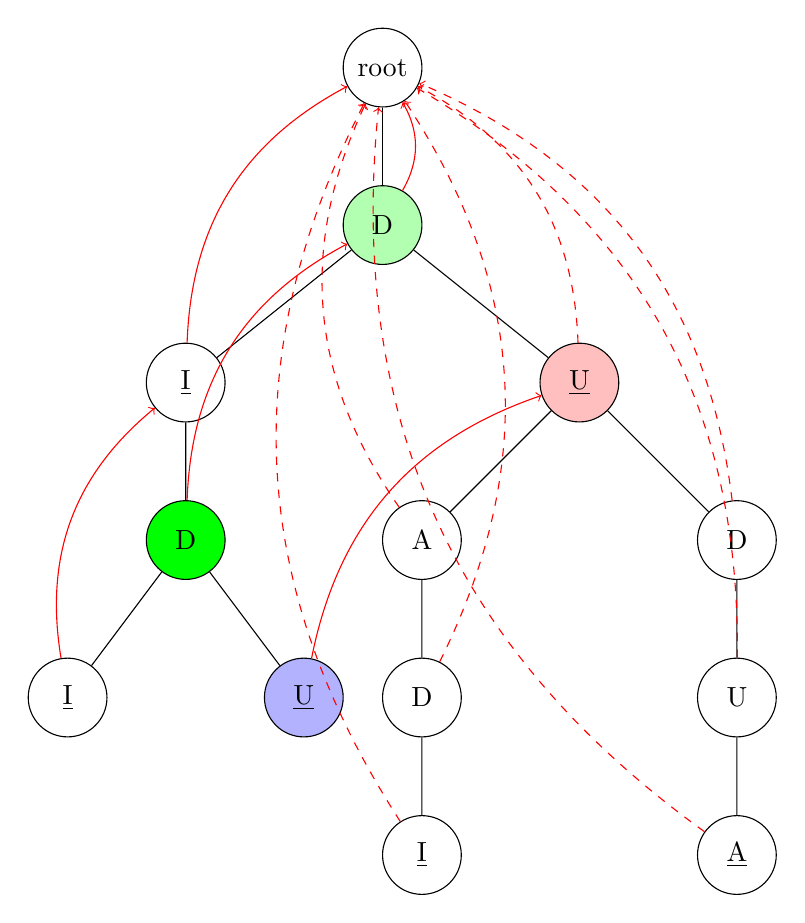
\begin{tikzpicture}[
        level 1/.style={sibling distance=6cm, level distance=2cm},
        level 2/.style={sibling distance=5cm, level distance=2cm},
        level 3/.style={sibling distance=4cm, level distance=2cm},
        level 4/.style={sibling distance=3cm, level distance=2cm},
        level 5/.style={sibling distance=2cm, level distance=2cm},
        level 6/.style={sibling distance=2cm, level distance=2ccm},
        every node/.style={circle, draw, minimum size=1cm}
    ]
        % Vẽ cây chính
        \node (root) {root}
            child { node [fill=green!30](D1) {D}
                child { node (I) {\underline{I}}
                    child { node [fill=green](D2) {D}
                        child { node (I2) {\underline{I}} }
                        child { node [fill=blue!30](U2) {\underline{U}} }
                    }
                }
                child { node [fill=pink](U1) {\underline{U}}
                    child { node (A2) {A}
                        child { node (D4) {D}
                            child { node (I3) {\underline{I}} }
                        }
                    }
                    child { node (D3) {D}
                        child { node (U3) {U}
                            child { node (A) {\underline{A}} }
                        }
                    }
                }
            };

        % Thêm các liên kết về gốc
        \draw[red, ->] (D1) to[bend right] (root);
        \draw[red, ->] (I) to[bend left] (root);
        \draw[red, ->] (I2) to[bend left] (I);
        \draw[red, ->] (D2) to[bend left] (D1);
        \draw[red, dashed, ->] (U1) to[bend right] (root);
        \draw[red, dashed, ->] (D3) to[bend right] (root);
        \draw[red, ->] (U2) to[bend left] (U1);
        \draw[red, dashed, ->] (A) to[bend left] (root);
        \draw[red, dashed, ->] (A2) to[bend left] (root);
        \draw[red, dashed, ->] (D4) to[bend right] (root);
        \draw[red, dashed, ->] (I3) to[bend left] (root);
        \draw[red, dashed, ->] (U3) to[bend right] (root);
    \end{tikzpicture}

\end{center}
Travel to node U. The parent of this node is node D. 
    
The suffix link of node D points to the other node D. 

The other node D has node U as its child so the suffix link is now pointing to that node.
\pagebreak

\textbf{Step 6:}
\begin{center}
    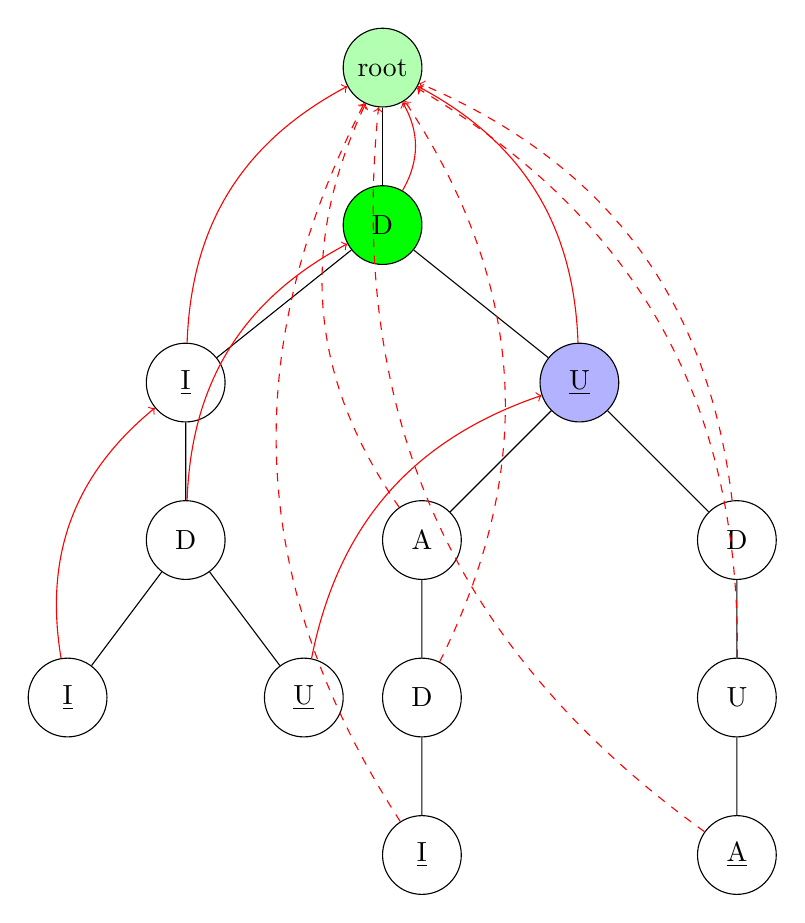
\begin{tikzpicture}[
        level 1/.style={sibling distance=6cm, level distance=2cm},
        level 2/.style={sibling distance=5cm, level distance=2cm},
        level 3/.style={sibling distance=4cm, level distance=2cm},
        level 4/.style={sibling distance=3cm, level distance=2cm},
        level 5/.style={sibling distance=2cm, level distance=2cm},
        level 6/.style={sibling distance=2cm, level distance=2ccm},
        every node/.style={circle, draw, minimum size=1cm}
    ]
        % Vẽ cây chính
        \node [fill=green!30](root) {root}
            child { node [fill=green](D1) {D}
                child { node (I) {\underline{I}}
                    child { node (D2) {D}
                        child { node (I2) {\underline{I}} }
                        child { node (U2) {\underline{U}} }
                    }
                }
                child { node [fill=blue!30](U1) {\underline{U}}
                    child { node (A2) {A}
                        child { node (D4) {D}
                            child { node (I3) {\underline{I}} }
                        }
                    }
                    child { node (D3) {D}
                        child { node (U3) {U}
                            child { node (A) {\underline{A}} }
                        }
                    }
                }
            };

        % Thêm các liên kết về gốc
        \draw[red, ->] (D1) to[bend right] (root);
        \draw[red, ->] (I) to[bend left] (root);
        \draw[red, ->] (I2) to[bend left] (I);
        \draw[red, ->] (D2) to[bend left] (D1);
        \draw[red, ->] (U1) to[bend right] (root);
        \draw[red, dashed, ->] (D3) to[bend right] (root);
        \draw[red, ->] (U2) to[bend left] (U1);
        \draw[red, dashed, ->] (A) to[bend left] (root);
        \draw[red, dashed, ->] (A2) to[bend left] (root);
        \draw[red, dashed, ->] (D4) to[bend right] (root);
        \draw[red, dashed, ->] (I3) to[bend left] (root);
        \draw[red, dashed, ->] (U3) to[bend right] (root);
    \end{tikzpicture}

\end{center}
Travel to node U. The parent of this node is node D. 
    
The suffix link of node D points to the root. 
    
The root doesn't have node U as its child node so we do nothing.
\pagebreak

\textbf{Step 7:}
\begin{center}
    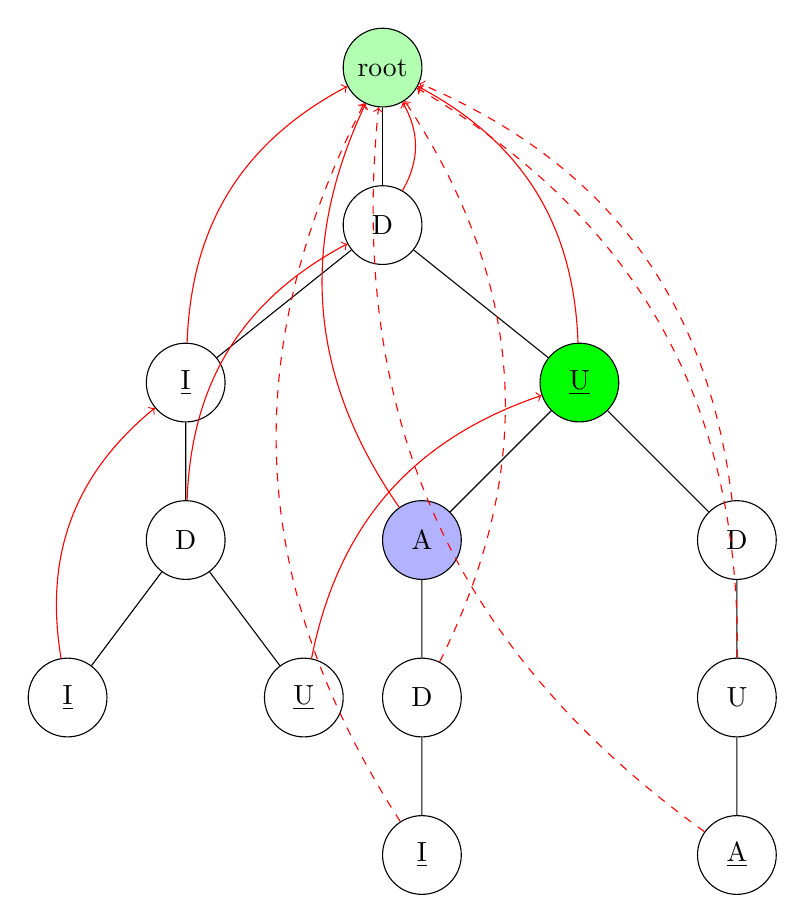
\begin{tikzpicture}[
        level 1/.style={sibling distance=6cm, level distance=2cm},
        level 2/.style={sibling distance=5cm, level distance=2cm},
        level 3/.style={sibling distance=4cm, level distance=2cm},
        level 4/.style={sibling distance=3cm, level distance=2cm},
        level 5/.style={sibling distance=2cm, level distance=2cm},
        level 6/.style={sibling distance=2cm, level distance=2ccm},
        every node/.style={circle, draw, minimum size=1cm}
    ]
        % Vẽ cây chính
        \node [fill=green!30](root) {root}
            child { node (D1) {D}
                child { node (I) {\underline{I}}
                    child { node (D2) {D}
                        child { node (I2) {\underline{I}} }
                        child { node (U2) {\underline{U}} }
                    }
                }
                child { node [fill=green](U1) {\underline{U}}
                    child { node [fill=blue!30](A2) {A}
                        child { node (D4) {D}
                            child { node (I3) {\underline{I}} }
                        }
                    }
                    child { node (D3) {D}
                        child { node (U3) {U}
                            child { node (A) {\underline{A}} }
                        }
                    }
                }
            };

        % Thêm các liên kết về gốc
        \draw[red, ->] (D1) to[bend right] (root);
        \draw[red, ->] (I) to[bend left] (root);
        \draw[red, ->] (I2) to[bend left] (I);
        \draw[red, ->] (D2) to[bend left] (D1);
        \draw[red, ->] (U1) to[bend right] (root);
        \draw[red, dashed, ->] (D3) to[bend right] (root);
        \draw[red, ->] (U2) to[bend left] (U1);
        \draw[red, dashed, ->] (A) to[bend left] (root);
        \draw[red, ->] (A2) to[bend left] (root);
        \draw[red, dashed, ->] (D4) to[bend right] (root);
        \draw[red, dashed, ->] (I3) to[bend left] (root);
        \draw[red, dashed, ->] (U3) to[bend right] (root);
    \end{tikzpicture}

\end{center}
Travel to node A. The parent of this node is node U. 
    
The suffix link of node U points to the root. 
    
The root doesn't have node A as its child node so we do nothing.
\pagebreak

\textbf{Step 8:}
\begin{center}
    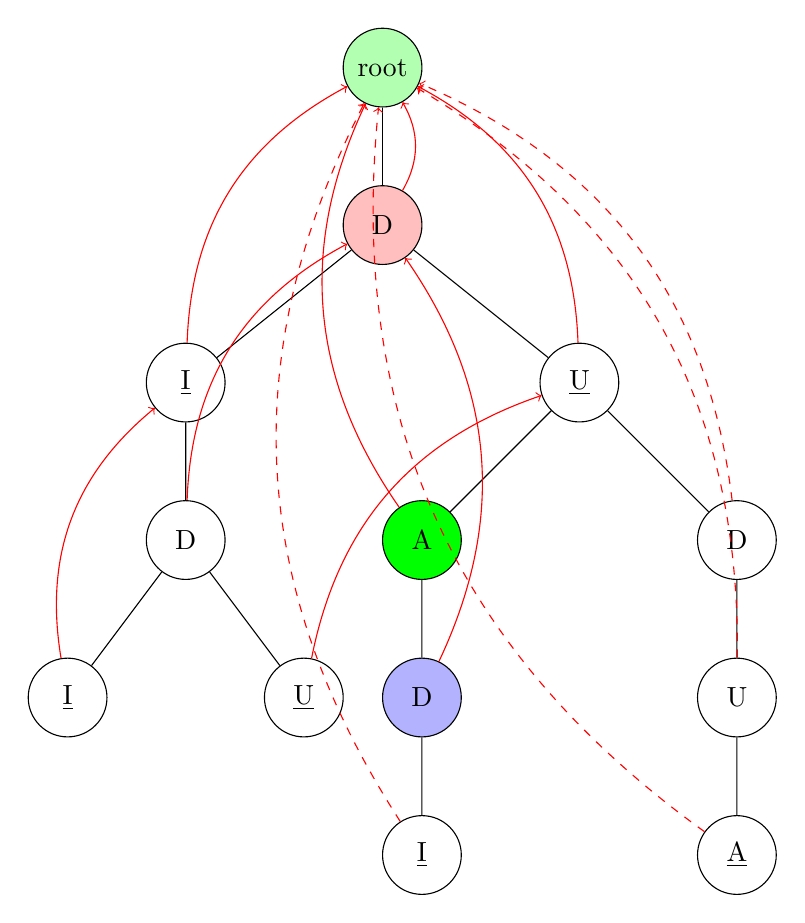
\begin{tikzpicture}[
        level 1/.style={sibling distance=6cm, level distance=2cm},
        level 2/.style={sibling distance=5cm, level distance=2cm},
        level 3/.style={sibling distance=4cm, level distance=2cm},
        level 4/.style={sibling distance=3cm, level distance=2cm},
        level 5/.style={sibling distance=2cm, level distance=2cm},
        level 6/.style={sibling distance=2cm, level distance=2ccm},
        every node/.style={circle, draw, minimum size=1cm}
    ]
        % Vẽ cây chính
        \node [fill=green!30](root) {root}
            child { node [fill=pink](D1) {D}
                child { node (I) {\underline{I}}
                    child { node (D2) {D}
                        child { node (I2) {\underline{I}} }
                        child { node (U2) {\underline{U}} }
                    }
                }
                child { node (U1) {\underline{U}}
                    child { node [fill=green](A2) {A}
                        child { node [fill=blue!30](D4) {D}
                            child { node (I3) {\underline{I}} }
                        }
                    }
                    child { node (D3) {D}
                        child { node (U3) {U}
                            child { node (A) {\underline{A}} }
                        }
                    }
                }
            };

        % Thêm các liên kết về gốc
        \draw[red, ->] (D1) to[bend right] (root);
        \draw[red, ->] (I) to[bend left] (root);
        \draw[red, ->] (I2) to[bend left] (I);
        \draw[red, ->] (D2) to[bend left] (D1);
        \draw[red, ->] (U1) to[bend right] (root);
        \draw[red, dashed, ->] (D3) to[bend right] (root);
        \draw[red, ->] (U2) to[bend left] (U1);
        \draw[red, dashed, ->] (A) to[bend left] (root);
        \draw[red, ->] (A2) to[bend left] (root);
        \draw[red, ->] (D4) to[bend right] (D1);
        \draw[red, dashed, ->] (I3) to[bend left] (root);
        \draw[red, dashed, ->] (U3) to[bend right] (root);
    \end{tikzpicture}

\end{center}
Travel to node D. The parent of this node is node A. 
    
The suffix link of node A points to the root. 
    
The root has node D as its child node so the suffix link is now pointing to that node.
\pagebreak

\textbf{Step 9:}
\begin{center}
    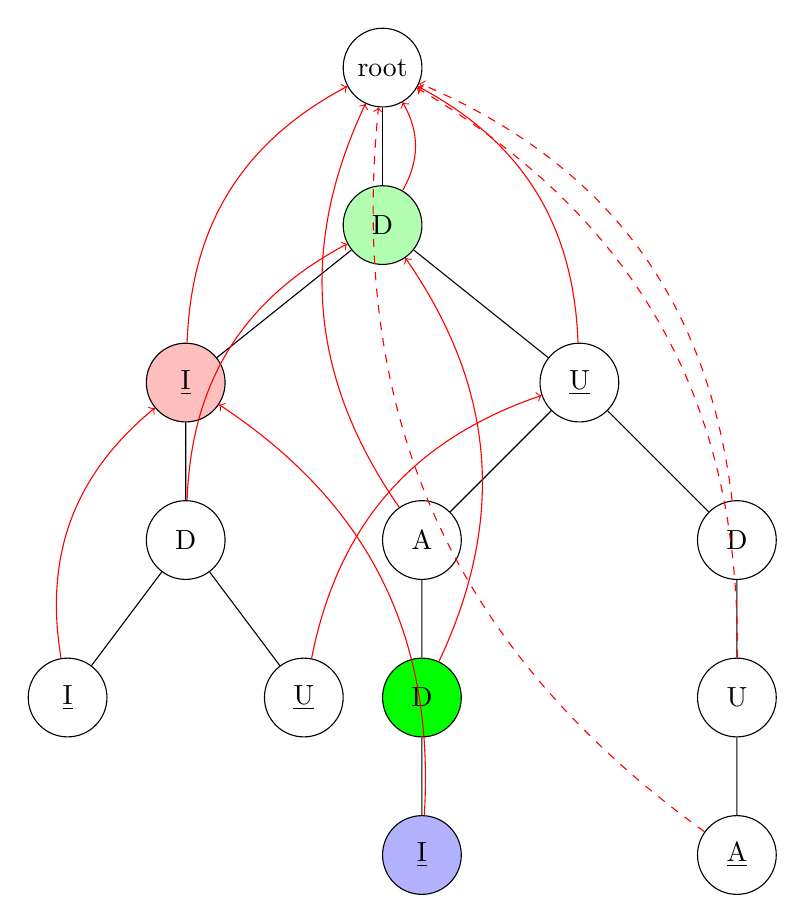
\begin{tikzpicture}[
        level 1/.style={sibling distance=6cm, level distance=2cm},
        level 2/.style={sibling distance=5cm, level distance=2cm},
        level 3/.style={sibling distance=4cm, level distance=2cm},
        level 4/.style={sibling distance=3cm, level distance=2cm},
        level 5/.style={sibling distance=2cm, level distance=2cm},
        level 6/.style={sibling distance=2cm, level distance=2ccm},
        every node/.style={circle, draw, minimum size=1cm}
    ]
        % Vẽ cây chính
        \node (root) {root}
            child { node [fill=green!30](D1) {D}
                child { node [fill=pink](I) {\underline{I}}
                    child { node (D2) {D}
                        child { node (I2) {\underline{I}} }
                        child { node (U2) {\underline{U}} }
                    }
                }
                child { node (U1) {\underline{U}}
                    child { node (A2) {A}
                        child { node [fill=green](D4) {D}
                            child { node [fill=blue!30](I3) {\underline{I}} }
                        }
                    }
                    child { node (D3) {D}
                        child { node (U3) {U}
                            child { node (A) {\underline{A}} }
                        }
                    }
                }
            };

        % Thêm các liên kết về gốc
        \draw[red, ->] (D1) to[bend right] (root);
        \draw[red, ->] (I) to[bend left] (root);
        \draw[red, ->] (I2) to[bend left] (I);
        \draw[red, ->] (D2) to[bend left] (D1);
        \draw[red, ->] (U1) to[bend right] (root);
        \draw[red, dashed, ->] (D3) to[bend right] (root);
        \draw[red, ->] (U2) to[bend left] (U1);
        \draw[red, dashed, ->] (A) to[bend left] (root);
        \draw[red, ->] (A2) to[bend left] (root);
        \draw[red, ->] (D4) to[bend right] (D1);
        \draw[red, ->] (I3) to[bend right] (I);
        \draw[red, dashed, ->] (U3) to[bend right] (root);
    \end{tikzpicture}

\end{center}
Travel to node I. The parent of this node is node I. 
    
The suffix link of node D points to the other node D. 
    
The other node D has node I as its child node so the suffix link is now pointing to that node.
\pagebreak

\textbf{Step 10:}
\begin{center}
    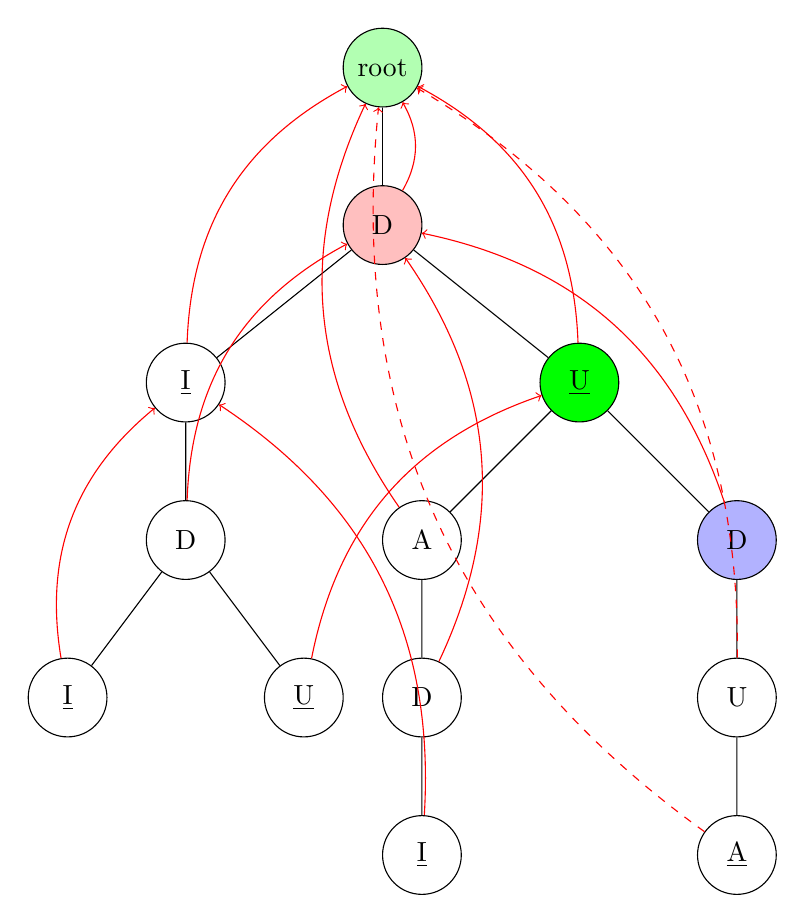
\begin{tikzpicture}[
        level 1/.style={sibling distance=6cm, level distance=2cm},
        level 2/.style={sibling distance=5cm, level distance=2cm},
        level 3/.style={sibling distance=4cm, level distance=2cm},
        level 4/.style={sibling distance=3cm, level distance=2cm},
        level 5/.style={sibling distance=2cm, level distance=2cm},
        level 6/.style={sibling distance=2cm, level distance=2ccm},
        every node/.style={circle, draw, minimum size=1cm}
    ]
        % Vẽ cây chính
        \node [fill=green!30](root) {root}
            child { node [fill=pink](D1) {D}
                child { node (I) {\underline{I}}
                    child { node (D2) {D}
                        child { node (I2) {\underline{I}} }
                        child { node (U2) {\underline{U}} }
                    }
                }
                child { node [fill=green](U1) {\underline{U}}
                    child { node (A2) {A}
                        child { node (D4) {D}
                            child { node (I3) {\underline{I}} }
                        }
                    }
                    child { node [fill=blue!30](D3) {D}
                        child { node (U3) {U}
                            child { node (A) {\underline{A}} }
                        }
                    }
                }
            };

        % Thêm các liên kết về gốc
        \draw[red, ->] (D1) to[bend right] (root);
        \draw[red, ->] (I) to[bend left] (root);
        \draw[red, ->] (I2) to[bend left] (I);
        \draw[red, ->] (D2) to[bend left] (D1);
        \draw[red, ->] (U1) to[bend right] (root);
        \draw[red, ->] (D3) to[bend right] (D1);
        \draw[red, ->] (U2) to[bend left] (U1);
        \draw[red, dashed, ->] (A) to[bend left] (root);
        \draw[red, ->] (A2) to[bend left] (root);
        \draw[red, ->] (D4) to[bend right] (D1);
        \draw[red, ->] (I3) to[bend right] (I);
        \draw[red, dashed, ->] (U3) to[bend right] (root);
    \end{tikzpicture}

\end{center}
Travel to node D. The parent of this node is node U. 
    
The suffix link of node U points to the root. 
    
The root has node D as its child node so the suffix link is now pointing to that node.
\pagebreak

\textbf{Step 11:}
\begin{center}
    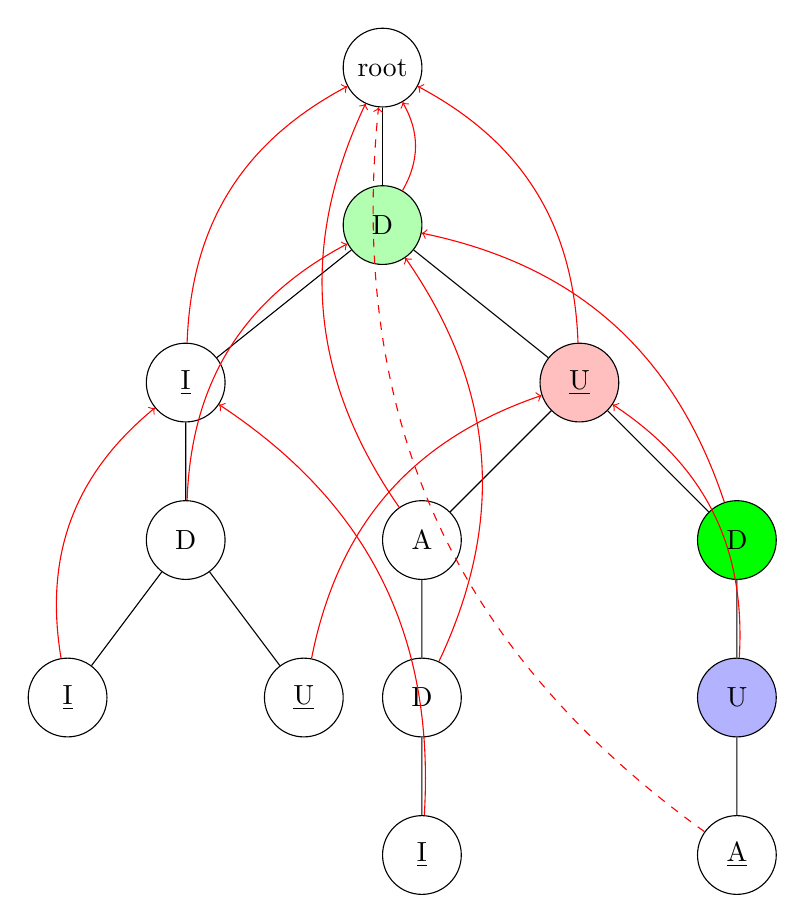
\begin{tikzpicture}[
        level 1/.style={sibling distance=6cm, level distance=2cm},
        level 2/.style={sibling distance=5cm, level distance=2cm},
        level 3/.style={sibling distance=4cm, level distance=2cm},
        level 4/.style={sibling distance=3cm, level distance=2cm},
        level 5/.style={sibling distance=2cm, level distance=2cm},
        level 6/.style={sibling distance=2cm, level distance=2ccm},
        every node/.style={circle, draw, minimum size=1cm}
    ]
        % Vẽ cây chính
        \node (root) {root}
            child { node [fill=green!30](D1) {D}
                child { node (I) {\underline{I}}
                    child { node (D2) {D}
                        child { node (I2) {\underline{I}} }
                        child { node (U2) {\underline{U}} }
                    }
                }
                child { node [fill=pink](U1) {\underline{U}}
                    child { node (A2) {A}
                        child { node (D4) {D}
                            child { node (I3) {\underline{I}} }
                        }
                    }
                    child { node [fill=green](D3) {D}
                        child { node[fill=blue!30] (U3) {U}
                            child { node (A) {\underline{A}} }
                        }
                    }
                }
            };

        % Thêm các liên kết về gốc
        \draw[red, ->] (D1) to[bend right] (root);
        \draw[red, ->] (I) to[bend left] (root);
        \draw[red, ->] (I2) to[bend left] (I);
        \draw[red, ->] (D2) to[bend left] (D1);
        \draw[red, ->] (U1) to[bend right] (root);
        \draw[red, ->] (D3) to[bend right] (D1);
        \draw[red, ->] (U2) to[bend left] (U1);
        \draw[red, dashed, ->] (A) to[bend left] (root);
        \draw[red, ->] (A2) to[bend left] (root);
        \draw[red, ->] (D4) to[bend right] (D1);
        \draw[red, ->] (I3) to[bend right] (I);
        \draw[red, ->] (U3) to[bend right] (U1);
    \end{tikzpicture}

\end{center}
Travel to node U. The parent of this node is node D. 
    
The suffix link of node D points to the other node D. 
    
The other node D has node U as its child node so the suffix link is now pointing to that node.
\pagebreak

\textbf{Step 12:}
\begin{center}
    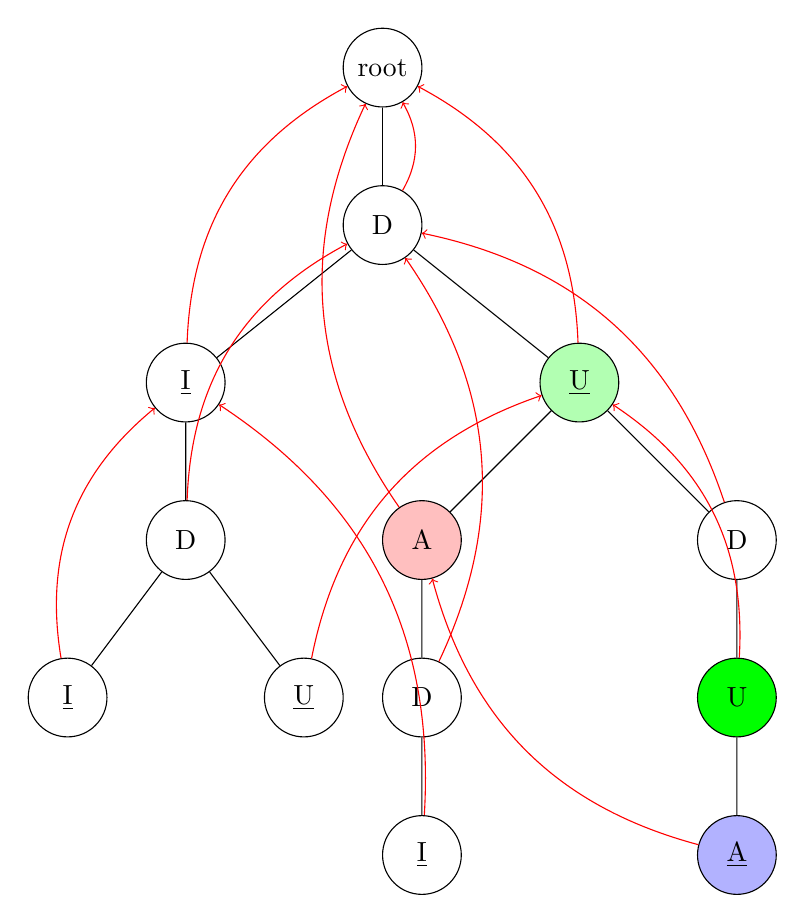
\begin{tikzpicture}[
        level 1/.style={sibling distance=6cm, level distance=2cm},
        level 2/.style={sibling distance=5cm, level distance=2cm},
        level 3/.style={sibling distance=4cm, level distance=2cm},
        level 4/.style={sibling distance=3cm, level distance=2cm},
        level 5/.style={sibling distance=2cm, level distance=2cm},
        level 6/.style={sibling distance=2cm, level distance=2ccm},
        every node/.style={circle, draw, minimum size=1cm}
    ]
        % Vẽ cây chính
        \node (root) {root}
            child { node (D1) {D}
                child { node (I) {\underline{I}}
                    child { node (D2) {D}
                        child { node (I2) {\underline{I}} }
                        child { node (U2) {\underline{U}} }
                    }
                }
                child { node [fill=green!30](U1) {\underline{U}}
                    child { node [fill=pink](A2) {A}
                        child { node (D4) {D}
                            child { node (I3) {\underline{I}} }
                        }
                    }
                    child { node (D3) {D}
                        child { node[fill=green] (U3) {U}
                            child { node [fill=blue!30](A) {\underline{A}} }
                        }
                    }
                }
            };

        % Thêm các liên kết về gốc
        \draw[red, ->] (D1) to[bend right] (root);
        \draw[red, ->] (I) to[bend left] (root);
        \draw[red, ->] (I2) to[bend left] (I);
        \draw[red, ->] (D2) to[bend left] (D1);
        \draw[red, ->] (U1) to[bend right] (root);
        \draw[red, ->] (D3) to[bend right] (D1);
        \draw[red, ->] (U2) to[bend left] (U1);
        \draw[red, ->] (A) to[bend left] (A2);
        \draw[red, ->] (A2) to[bend left] (root);
        \draw[red, ->] (D4) to[bend right] (D1);
        \draw[red, ->] (I3) to[bend right] (I);
        \draw[red, ->] (U3) to[bend right] (U1);
    \end{tikzpicture}

\end{center}
Travel to node A. The parent of this node is node U. 
    
The suffix link of node U points to the other node U. 
    
The other node U has node A as its child node so the suffix link is now pointing to that node.
\pagebreak
\subsubsection*{Result}
\begin{center}
    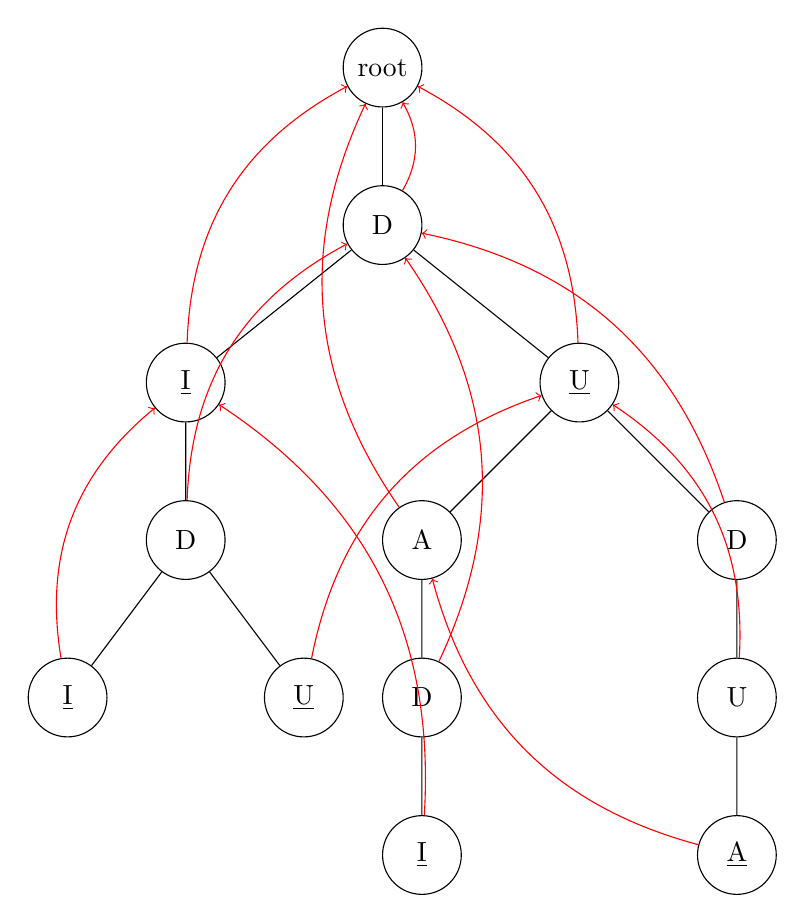
\begin{tikzpicture}[
        level 1/.style={sibling distance=6cm, level distance=2cm},
        level 2/.style={sibling distance=5cm, level distance=2cm},
        level 3/.style={sibling distance=4cm, level distance=2cm},
        level 4/.style={sibling distance=3cm, level distance=2cm},
        level 5/.style={sibling distance=2cm, level distance=2cm},
        level 6/.style={sibling distance=2cm, level distance=2ccm},
        every node/.style={circle, draw, minimum size=1cm}
    ]
        % Vẽ cây chính
        \node (root) {root}
            child { node (D1) {D}
                child { node (I) {\underline{I}}
                    child { node (D2) {D}
                        child { node (I2) {\underline{I}} }
                        child { node (U2) {\underline{U}} }
                    }
                }
                child { node (U1) {\underline{U}}
                    child { node (A2) {A}
                        child { node (D4) {D}
                            child { node (I3) {\underline{I}} }
                        }
                    }
                    child { node (D3) {D}
                        child { node (U3) {U}
                            child { node (A) {\underline{A}} }
                        }
                    }
                }
            };

        % Thêm các liên kết về gốc
        \draw[red, ->] (D1) to[bend right] (root);
        \draw[red, ->] (I) to[bend left] (root);
        \draw[red, ->] (I2) to[bend left] (I);
        \draw[red, ->] (D2) to[bend left] (D1);
        \draw[red, ->] (U1) to[bend right] (root);
        \draw[red, ->] (D3) to[bend right] (D1);
        \draw[red, ->] (U2) to[bend left] (U1);
        \draw[red, ->] (A) to[bend left] (A2);
        \draw[red, ->] (A2) to[bend left] (root);
        \draw[red, ->] (D4) to[bend right] (D1);
        \draw[red, ->] (I3) to[bend right] (I);
        \draw[red, ->] (U3) to[bend right] (U1);
    \end{tikzpicture}
\end{center}
\subsection{Matching/ Searching process}
At this process, we use the character at the position i of the text to travel through trie respectively.

At position i, if the current has the child text[i], we will travel to that child node. Otherwise, we use the suffix link to trace back to the other node to check whether that node has that child text[i]. This procedure repeats until there is a child node text[i] or the node is the root. If the node is the root, the searching process will stop. But there is a child node text[i], we will travel to that node and continue the procedure. 

After travel to that node, if the node is the end of a pattern and we have not counted that pattern, so we count it. Then we trace back using the suffix link procedure until the node is the root to check that all the prefixes are the end of any pattern or not. If there is the end of the pattern and it has not been counted, we count it. 
\pagebreak
\subsubsection*{Source code}
\lstinputlisting[language=C++]{code/traceBack.cpp}
\pagebreak
\subsubsection*{Step by step}
\textbf{Step 1:}
\begin{center}

    \begin{table}[H]
    \centering
    \begin{tabular}{|c|c|c|c|c|c|c|c|c|c|}
    \hline
    pos   & i &   &   &   &   &   &   &   &   \\ \hline
    text  & D & I & D & U & D & U & A & D & I \\ \hline
    \end{tabular}
    \end{table}
    
    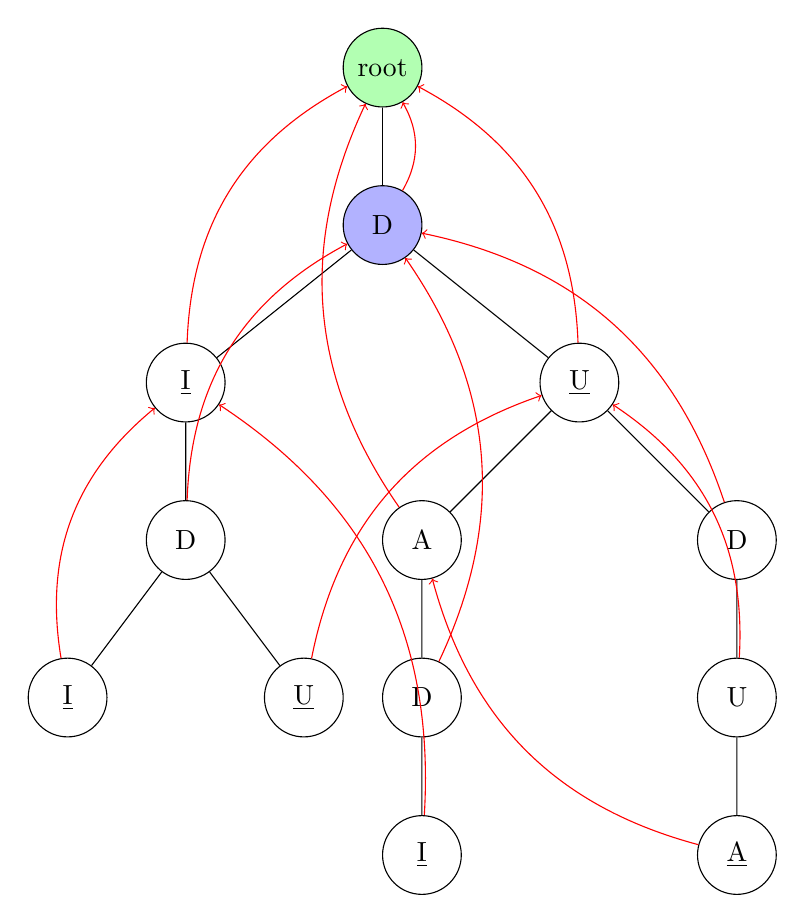
\begin{tikzpicture}[
        level 1/.style={sibling distance=6cm, level distance=2cm},
        level 2/.style={sibling distance=5cm, level distance=2cm},
        level 3/.style={sibling distance=4cm, level distance=2cm},
        level 4/.style={sibling distance=3cm, level distance=2cm},
        level 5/.style={sibling distance=2cm, level distance=2cm},
        level 6/.style={sibling distance=2cm, level distance=2ccm},
        every node/.style={circle, draw, minimum size=1cm}
    ]
        % Vẽ cây chính
        \node [fill=green!30](root) {root}
            child { node [fill=blue!30](D1) {D}
                child { node (I) {\underline{I}}
                    child { node (D2) {D}
                        child { node (I2) {\underline{I}} }
                        child { node (U2) {\underline{U}} }
                    }
                }
                child { node (U1) {\underline{U}}
                    child { node (A2) {A}
                        child { node (D4) {D}
                            child { node (I3) {\underline{I}} }
                        }
                    }
                    child { node (D3) {D}
                        child { node (U3) {U}
                            child { node (A) {\underline{A}} }
                        }
                    }
                }
            };

        % Thêm các liên kết về gốc
        \draw[red, ->] (D1) to[bend right] (root);
        \draw[red, ->] (I) to[bend left] (root);
        \draw[red, ->] (I2) to[bend left] (I);
        \draw[red, ->] (D2) to[bend left] (D1);
        \draw[red, ->] (U1) to[bend right] (root);
        \draw[red, ->] (D3) to[bend right] (D1);
        \draw[red, ->] (U2) to[bend left] (U1);
        \draw[red, ->] (A) to[bend left] (A2);
        \draw[red, ->] (A2) to[bend left] (root);
        \draw[red, ->] (D4) to[bend right] (D1);
        \draw[red, ->] (I3) to[bend right] (I);
        \draw[red, ->] (U3) to[bend right] (U1);
    \end{tikzpicture}

\end{center}
The number of patterns that occur in the text: 0.

Now text[i] = D, we travel to node D from the root. Because node D is not the end of any patterns, we do nothing in this node. We trace back to the node the suffix link of this node points at, which is the root. Because this is the root, we stop the procedure.
\pagebreak

\textbf{Step 2:}
\begin{center}

    \begin{table}[H]
    \centering
    \begin{tabular}{|c|c|c|c|c|c|c|c|c|c|}
    \hline
    pos   &   & i &   &   &   &   &   &   &   \\ \hline
    text  & D & I & D & U & D & U & A & D & I \\ \hline
    \end{tabular}
    \end{table}
    
    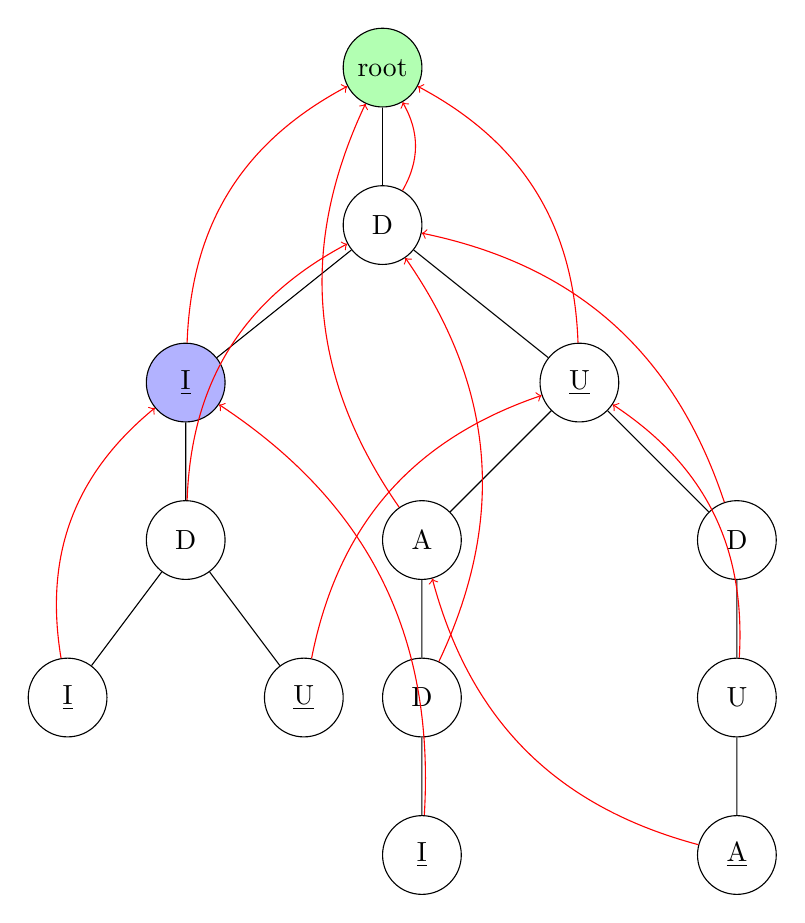
\begin{tikzpicture}[
        level 1/.style={sibling distance=6cm, level distance=2cm},
        level 2/.style={sibling distance=5cm, level distance=2cm},
        level 3/.style={sibling distance=4cm, level distance=2cm},
        level 4/.style={sibling distance=3cm, level distance=2cm},
        level 5/.style={sibling distance=2cm, level distance=2cm},
        level 6/.style={sibling distance=2cm, level distance=2ccm},
        every node/.style={circle, draw, minimum size=1cm}
    ]
        % Vẽ cây chính
        \node [fill=green!30](root) {root}
            child { node (D1) {D}
                child { node [fill=blue!30](I) {\underline{I}}
                    child { node (D2) {D}
                        child { node (I2) {\underline{I}} }
                        child { node (U2) {\underline{U}} }
                    }
                }
                child { node (U1) {\underline{U}}
                    child { node (A2) {A}
                        child { node (D4) {D}
                            child { node (I3) {\underline{I}} }
                        }
                    }
                    child { node (D3) {D}
                        child { node (U3) {U}
                            child { node (A) {\underline{A}} }
                        }
                    }
                }
            };

        % Thêm các liên kết về gốc
        \draw[red, ->] (D1) to[bend right] (root);
        \draw[red, ->] (I) to[bend left] (root);
        \draw[red, ->] (I2) to[bend left] (I);
        \draw[red, ->] (D2) to[bend left] (D1);
        \draw[red, ->] (U1) to[bend right] (root);
        \draw[red, ->] (D3) to[bend right] (D1);
        \draw[red, ->] (U2) to[bend left] (U1);
        \draw[red, ->] (A) to[bend left] (A2);
        \draw[red, ->] (A2) to[bend left] (root);
        \draw[red, ->] (D4) to[bend right] (D1);
        \draw[red, ->] (I3) to[bend right] (I);
        \draw[red, ->] (U3) to[bend right] (U1);
    \end{tikzpicture}

\end{center}
Number of patterns that occur in the text: 1 (DI).

Now text[i] = I, we travel to node I from node D. Because node I is the end of a pattern DI and pattern have not been counted, the number of pattern that occur in the text is increased by 1. We trace back to the node the suffix of this node points at, which is the root, Because this is the root, we stop the procedure.
\pagebreak

\textbf{Step 3:}
\begin{center}

    \begin{table}[H]
    \centering
    \begin{tabular}{|c|c|c|c|c|c|c|c|c|c|}
    \hline
    pos   &   &   & i &   &   &   &   &   &   \\ \hline
    text  & D & I & D & U & D & U & A & D & I \\ \hline
    \end{tabular}
    \end{table}
    
    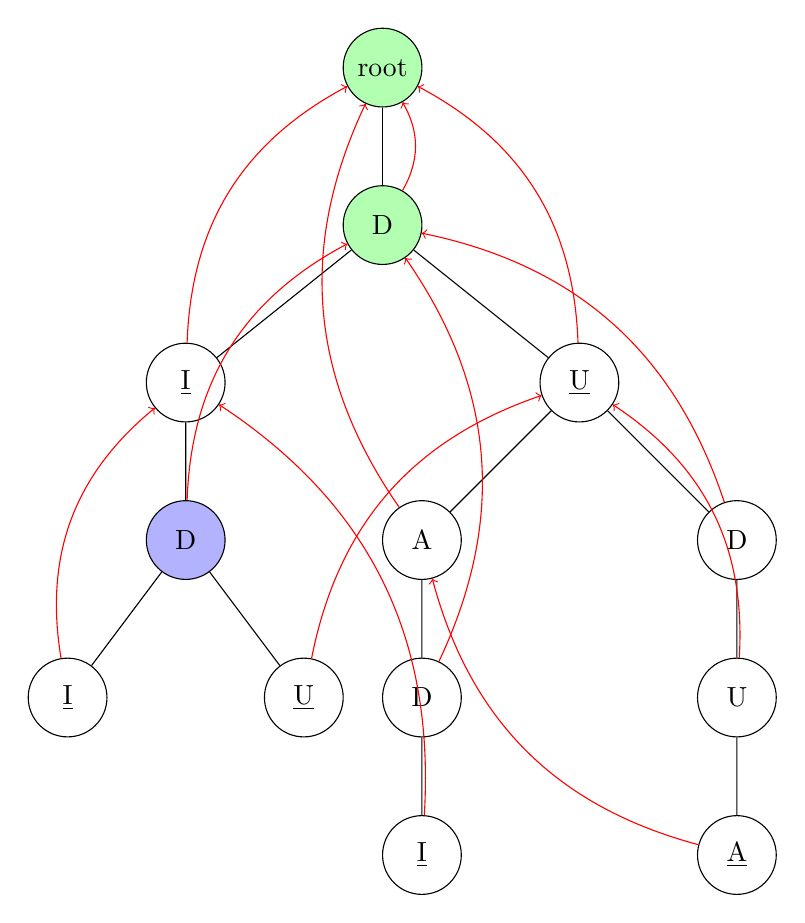
\begin{tikzpicture}[
        level 1/.style={sibling distance=6cm, level distance=2cm},
        level 2/.style={sibling distance=5cm, level distance=2cm},
        level 3/.style={sibling distance=4cm, level distance=2cm},
        level 4/.style={sibling distance=3cm, level distance=2cm},
        level 5/.style={sibling distance=2cm, level distance=2cm},
        level 6/.style={sibling distance=2cm, level distance=2ccm},
        every node/.style={circle, draw, minimum size=1cm}
    ]
        % Vẽ cây chính
        \node [fill=green!30](root) {root}
            child { node [fill=green!30](D1) {D}
                child { node (I) {\underline{I}}
                    child { node [fill=blue!30](D2) {D}
                        child { node (I2) {\underline{I}} }
                        child { node (U2) {\underline{U}} }
                    }
                }
                child { node (U1) {\underline{U}}
                    child { node (A2) {A}
                        child { node (D4) {D}
                            child { node (I3) {\underline{I}} }
                        }
                    }
                    child { node (D3) {D}
                        child { node (U3) {U}
                            child { node (A) {\underline{A}} }
                        }
                    }
                }
            };

        % Thêm các liên kết về gốc
        \draw[red, ->] (D1) to[bend right] (root);
        \draw[red, ->] (I) to[bend left] (root);
        \draw[red, ->] (I2) to[bend left] (I);
        \draw[red, ->] (D2) to[bend left] (D1);
        \draw[red, ->] (U1) to[bend right] (root);
        \draw[red, ->] (D3) to[bend right] (D1);
        \draw[red, ->] (U2) to[bend left] (U1);
        \draw[red, ->] (A) to[bend left] (A2);
        \draw[red, ->] (A2) to[bend left] (root);
        \draw[red, ->] (D4) to[bend right] (D1);
        \draw[red, ->] (I3) to[bend right] (I);
        \draw[red, ->] (U3) to[bend right] (U1);
    \end{tikzpicture}

\end{center}
Number of patterns that occur in the text: 1 (DI).

Now text[i] = D, we travel to node D from node I. Because node D is not the end of nay patterns, we do nothing. We trace back to the node the suffix link of this node points at, which is the other node D. Because node D is not the end of any pattern, we do nothing at this node. We trace back to the node the suffix link of this node points at, which is the root. Because this is the root, we stop the procedure.
\pagebreak

\textbf{Step 4:}
\begin{center}

    \begin{table}[H]
    \centering
    \begin{tabular}{|c|c|c|c|c|c|c|c|c|c|}
    \hline
    pos   &   &   &   & i &   &   &   &   &   \\ \hline
    text  & D & I & D & U & D & U & A & D & I \\ \hline
    \end{tabular}
    \end{table}
    
    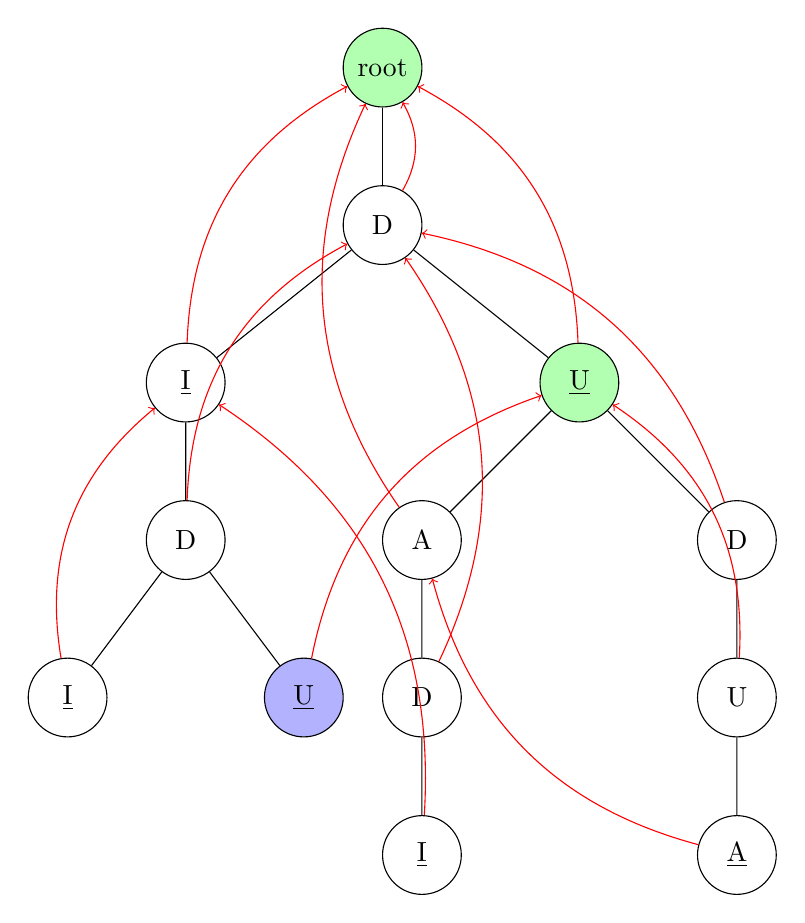
\begin{tikzpicture}[
        level 1/.style={sibling distance=6cm, level distance=2cm},
        level 2/.style={sibling distance=5cm, level distance=2cm},
        level 3/.style={sibling distance=4cm, level distance=2cm},
        level 4/.style={sibling distance=3cm, level distance=2cm},
        level 5/.style={sibling distance=2cm, level distance=2cm},
        level 6/.style={sibling distance=2cm, level distance=2ccm},
        every node/.style={circle, draw, minimum size=1cm}
    ]
        % Vẽ cây chính
        \node [fill=green!30](root) {root}
            child { node (D1) {D}
                child { node (I) {\underline{I}}
                    child { node (D2) {D}
                        child { node (I2) {\underline{I}} }
                        child { node [fill=blue!30](U2) {\underline{U}} }
                    }
                }
                child { node [fill=green!30](U1) {\underline{U}}
                    child { node (A2) {A}
                        child { node (D4) {D}
                            child { node (I3) {\underline{I}} }
                        }
                    }
                    child { node (D3) {D}
                        child { node (U3) {U}
                            child { node (A) {\underline{A}} }
                        }
                    }
                }
            };

        % Thêm các liên kết về gốc
        \draw[red, ->] (D1) to[bend right] (root);
        \draw[red, ->] (I) to[bend left] (root);
        \draw[red, ->] (I2) to[bend left] (I);
        \draw[red, ->] (D2) to[bend left] (D1);
        \draw[red, ->] (U1) to[bend right] (root);
        \draw[red, ->] (D3) to[bend right] (D1);
        \draw[red, ->] (U2) to[bend left] (U1);
        \draw[red, ->] (A) to[bend left] (A2);
        \draw[red, ->] (A2) to[bend left] (root);
        \draw[red, ->] (D4) to[bend right] (D1);
        \draw[red, ->] (I3) to[bend right] (I);
        \draw[red, ->] (U3) to[bend right] (U1);
    \end{tikzpicture}

\end{center}
Number of patterns that occur in the text: 3 (DI, DIDU, DU).

Now text[i] = I, we travel to node U from node D. Because node U is the end of a pattern DIDU and this pattern have not been counted, the number of patterns that occur in the text in increased by 1. We trace back to the node the suffix link of this node points at, which is the other node U. Because node U is the end of pattern DU and this pattern have not been counted, the number of patterns that occur in the text is increased by 1. We trace back to the node the suffix link of this node points at, which is the root. Because this is the root, we stop the procedure.
\pagebreak

\textbf{Step 5:}
\begin{center}

    \begin{table}[H]
    \centering
    \begin{tabular}{|c|c|c|c|c|c|c|c|c|c|}
    \hline
    pos   &   &   &   &   & i &   &   &   &   \\ \hline
    text  & D & I & D & U & D & U & A & D & I \\ \hline
    \end{tabular}
    \end{table}
    
    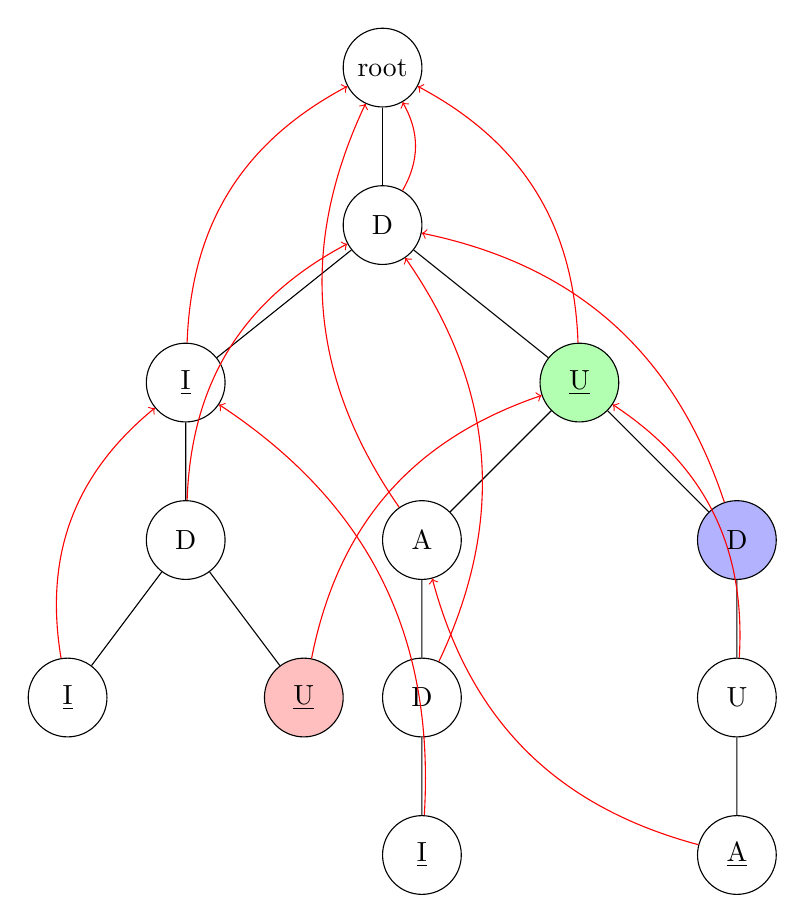
\begin{tikzpicture}[
        level 1/.style={sibling distance=6cm, level distance=2cm},
        level 2/.style={sibling distance=5cm, level distance=2cm},
        level 3/.style={sibling distance=4cm, level distance=2cm},
        level 4/.style={sibling distance=3cm, level distance=2cm},
        level 5/.style={sibling distance=2cm, level distance=2cm},
        level 6/.style={sibling distance=2cm, level distance=2ccm},
        every node/.style={circle, draw, minimum size=1cm}
    ]
        % Vẽ cây chính
        \node (root) {root}
            child { node (D1) {D}
                child { node (I) {\underline{I}}
                    child { node (D2) {D}
                        child { node (I2) {\underline{I}} }
                        child { node [fill=pink](U2) {\underline{U}} }
                    }
                }
                child { node [fill=green!30](U1) {\underline{U}}
                    child { node (A2) {A}
                        child { node (D4) {D}
                            child { node (I3) {\underline{I}} }
                        }
                    }
                    child { node [fill=blue!30](D3) {D}
                        child { node (U3) {U}
                            child { node (A) {\underline{A}} }
                        }
                    }
                }
            };

        % Thêm các liên kết về gốc
        \draw[red, ->] (D1) to[bend right] (root);
        \draw[red, ->] (I) to[bend left] (root);
        \draw[red, ->] (I2) to[bend left] (I);
        \draw[red, ->] (D2) to[bend left] (D1);
        \draw[red, ->] (U1) to[bend right] (root);
        \draw[red, ->] (D3) to[bend right] (D1);
        \draw[red, ->] (U2) to[bend left] (U1);
        \draw[red, ->] (A) to[bend left] (A2);
        \draw[red, ->] (A2) to[bend left] (root);
        \draw[red, ->] (D4) to[bend right] (D1);
        \draw[red, ->] (I3) to[bend right] (I);
        \draw[red, ->] (U3) to[bend right] (U1);
    \end{tikzpicture}

\end{center}
Number of patterns that occur in the text: 3 (DI, DIDU, DU).

Now text[i] = D, but node U doesn't have node child D we trace back to the node the suffix link of node U points at, which points to other node U. That node U has node child D so we travel to that node D.
\pagebreak

\textbf{Step 6:}
\begin{center}

    \begin{table}[H]
    \centering
    \begin{tabular}{|c|c|c|c|c|c|c|c|c|c|}
    \hline
    pos   &   &   &   &   & i &   &   &   &   \\ \hline
    text  & D & I & D & U & D & U & A & D & I \\ \hline
    \end{tabular}
    \end{table}
    
    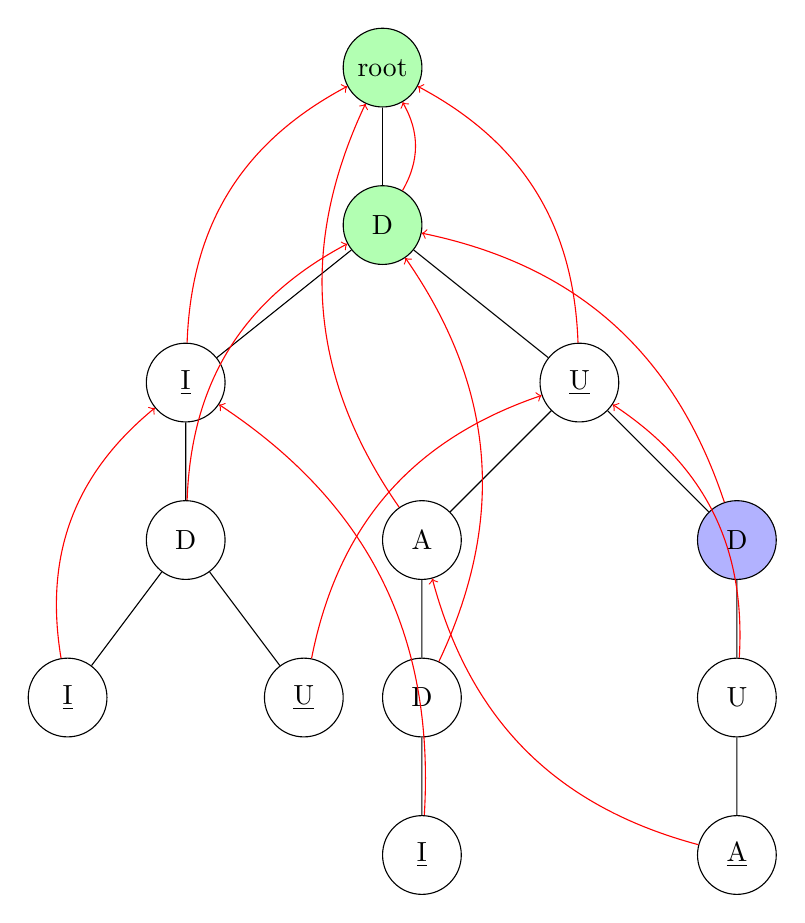
\begin{tikzpicture}[
        level 1/.style={sibling distance=6cm, level distance=2cm},
        level 2/.style={sibling distance=5cm, level distance=2cm},
        level 3/.style={sibling distance=4cm, level distance=2cm},
        level 4/.style={sibling distance=3cm, level distance=2cm},
        level 5/.style={sibling distance=2cm, level distance=2cm},
        level 6/.style={sibling distance=2cm, level distance=2ccm},
        every node/.style={circle, draw, minimum size=1cm}
    ]
        % Vẽ cây chính
        \node [fill=green!30](root) {root}
            child { node [fill=green!30](D1) {D}
                child { node (I) {\underline{I}}
                    child { node (D2) {D}
                        child { node (I2) {\underline{I}} }
                        child { node (U2) {\underline{U}} }
                    }
                }
                child { node (U1) {\underline{U}}
                    child { node (A2) {A}
                        child { node (D4) {D}
                            child { node (I3) {\underline{I}} }
                        }
                    }
                    child { node [fill=blue!30](D3) {D}
                        child { node (U3) {U}
                            child { node (A) {\underline{A}} }
                        }
                    }
                }
            };

        % Thêm các liên kết về gốc
        \draw[red, ->] (D1) to[bend right] (root);
        \draw[red, ->] (I) to[bend left] (root);
        \draw[red, ->] (I2) to[bend left] (I);
        \draw[red, ->] (D2) to[bend left] (D1);
        \draw[red, ->] (U1) to[bend right] (root);
        \draw[red, ->] (D3) to[bend right] (D1);
        \draw[red, ->] (U2) to[bend left] (U1);
        \draw[red, ->] (A) to[bend left] (A2);
        \draw[red, ->] (A2) to[bend left] (root);
        \draw[red, ->] (D4) to[bend right] (D1);
        \draw[red, ->] (I3) to[bend right] (I);
        \draw[red, ->] (U3) to[bend right] (U1);
    \end{tikzpicture}

\end{center}
Number of patterns that occur in the text: 3 (DI, DIDU, DU).

After travel to node D, node D is not the end of any pattern so we do nothing at this node. We trace back to the node the suffix link of this node points at, which is other node D. Because this node is not the end of any pattern, we do nothing on this node. We continue to trace back to the node the suffix link of this node points at, which is the root. Because this is the root, we stop the procedure.
\pagebreak

\textbf{Step 7:}
\begin{center}

    \begin{table}[H]
    \centering
    \begin{tabular}{|c|c|c|c|c|c|c|c|c|c|}
    \hline
    pos   &   &   &   &   &   & i &   &   &   \\ \hline
    text  & D & I & D & U & D & U & A & D & I \\ \hline
    \end{tabular}
    \end{table}
    
    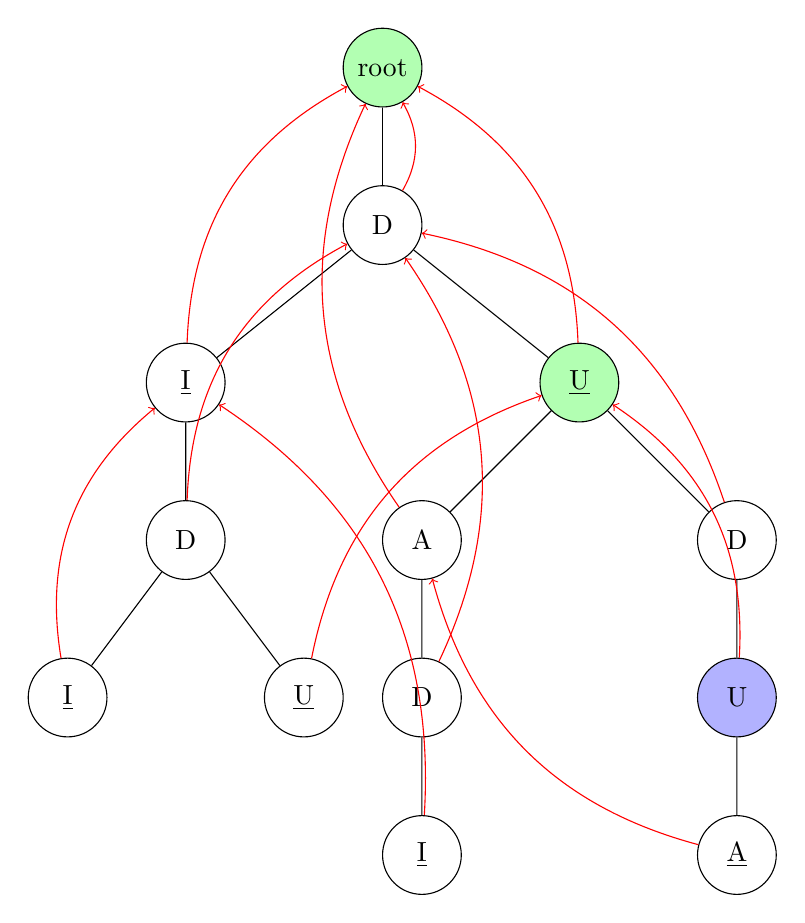
\begin{tikzpicture}[
        level 1/.style={sibling distance=6cm, level distance=2cm},
        level 2/.style={sibling distance=5cm, level distance=2cm},
        level 3/.style={sibling distance=4cm, level distance=2cm},
        level 4/.style={sibling distance=3cm, level distance=2cm},
        level 5/.style={sibling distance=2cm, level distance=2cm},
        level 6/.style={sibling distance=2cm, level distance=2ccm},
        every node/.style={circle, draw, minimum size=1cm}
    ]
        % Vẽ cây chính
        \node [fill=green!30](root) {root}
            child { node (D1) {D}
                child { node (I) {\underline{I}}
                    child { node (D2) {D}
                        child { node (I2) {\underline{I}} }
                        child { node (U2) {\underline{U}} }
                    }
                }
                child { node [fill=green!30](U1) {\underline{U}}
                    child { node (A2) {A}
                        child { node (D4) {D}
                            child { node (I3) {\underline{I}} }
                        }
                    }
                    child { node (D3) {D}
                        child { node [fill=blue!30](U3) {U}
                            child { node (A) {\underline{A}} }
                        }
                    }
                }
            };

        % Thêm các liên kết về gốc
        \draw[red, ->] (D1) to[bend right] (root);
        \draw[red, ->] (I) to[bend left] (root);
        \draw[red, ->] (I2) to[bend left] (I);
        \draw[red, ->] (D2) to[bend left] (D1);
        \draw[red, ->] (U1) to[bend right] (root);
        \draw[red, ->] (D3) to[bend right] (D1);
        \draw[red, ->] (U2) to[bend left] (U1);
        \draw[red, ->] (A) to[bend left] (A2);
        \draw[red, ->] (A2) to[bend left] (root);
        \draw[red, ->] (D4) to[bend right] (D1);
        \draw[red, ->] (I3) to[bend right] (I);
        \draw[red, ->] (U3) to[bend right] (U1);
    \end{tikzpicture}

\end{center}
Number of patterns that occur in the text: 3 (DI, DIDU, DU).

Now text[i] = U, we travel to node U from node D. Because this node is not the end of any pattern, we do nothing on this node. We trace back to the node the suffix link of this node points at, which is other node U. This other node U is the end of pattern DU but this pattern has already counted so we do nothing on this node. We countinue to trace back to the node the suffix of this node points at, which is the root. Because this is the root, we stop the procedure.
\pagebreak

\textbf{Step 8:}
\begin{center}

    \begin{table}[H]
    \centering
    \begin{tabular}{|c|c|c|c|c|c|c|c|c|c|}
    \hline
    pos   &   &   &   &   &   &   & i &   &   \\ \hline
    text  & D & I & D & U & D & U & A & D & I \\ \hline
    \end{tabular}
    \end{table}
    
    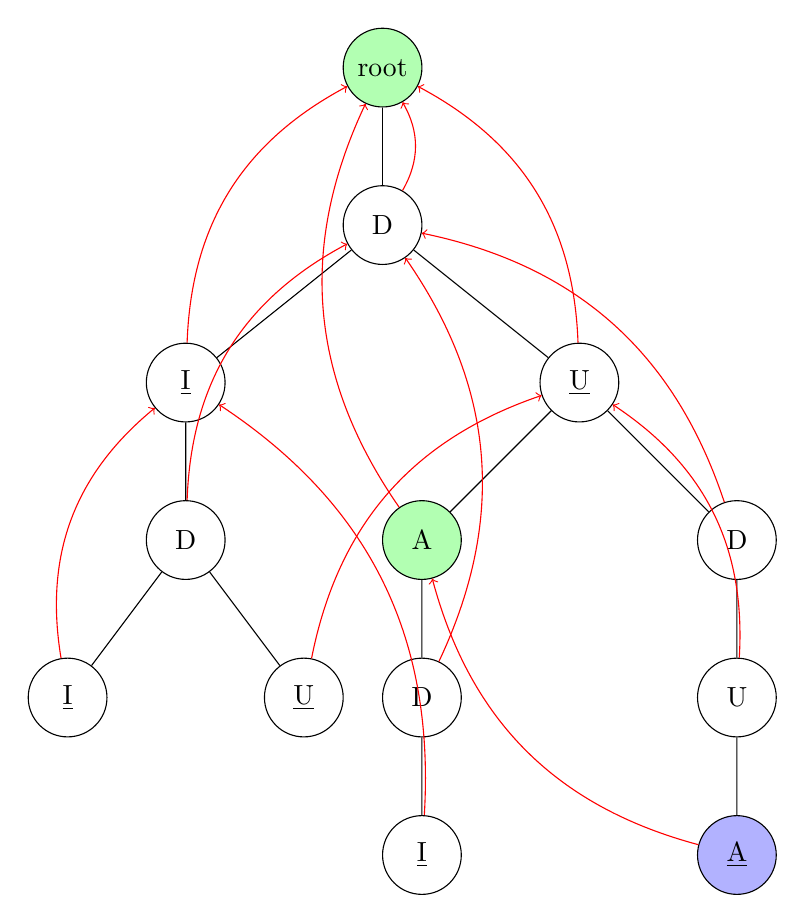
\begin{tikzpicture}[
        level 1/.style={sibling distance=6cm, level distance=2cm},
        level 2/.style={sibling distance=5cm, level distance=2cm},
        level 3/.style={sibling distance=4cm, level distance=2cm},
        level 4/.style={sibling distance=3cm, level distance=2cm},
        level 5/.style={sibling distance=2cm, level distance=2cm},
        level 6/.style={sibling distance=2cm, level distance=2ccm},
        every node/.style={circle, draw, minimum size=1cm}
    ]
        % Vẽ cây chính
        \node [fill=green!30](root) {root}
            child { node (D1) {D}
                child { node (I) {\underline{I}}
                    child { node (D2) {D}
                        child { node (I2) {\underline{I}} }
                        child { node (U2) {\underline{U}} }
                    }
                }
                child { node (U1) {\underline{U}}
                    child { node [fill=green!30](A2) {A}
                        child { node (D4) {D}
                            child { node (I3) {\underline{I}} }
                        }
                    }
                    child { node (D3) {D}
                        child { node (U3) {U}
                            child { node [fill=blue!30](A) {\underline{A}} }
                        }
                    }
                }
            };

        % Thêm các liên kết về gốc
        \draw[red, ->] (D1) to[bend right] (root);
        \draw[red, ->] (I) to[bend left] (root);
        \draw[red, ->] (I2) to[bend left] (I);
        \draw[red, ->] (D2) to[bend left] (D1);
        \draw[red, ->] (U1) to[bend right] (root);
        \draw[red, ->] (D3) to[bend right] (D1);
        \draw[red, ->] (U2) to[bend left] (U1);
        \draw[red, ->] (A) to[bend left] (A2);
        \draw[red, ->] (A2) to[bend left] (root);
        \draw[red, ->] (D4) to[bend right] (D1);
        \draw[red, ->] (I3) to[bend right] (I);
        \draw[red, ->] (U3) to[bend right] (U1);
    \end{tikzpicture}

\end{center}
Number of patterns that occur in the text: 4 (DI, DIDU, DU, DUDUA).

Now text[i] = A, we travel to node A from node U. Because this node is the end of pattern DUDUA and this pattern have not been counted, the number of patterns that occur in the text is increased by 1. We trace back to the node the suffix link of this node points at, which is other node A. This other node A is not the end of any pattern so we do nothing on this node. We countinue to trace back to the node the suffix of this node points at, which is the root. Because this is the root, we stop the procedure.
\pagebreak

\textbf{Step 9:}
\begin{center}

    \begin{table}[H]
    \centering
    \begin{tabular}{|c|c|c|c|c|c|c|c|c|c|}
    \hline
    pos   &   &   &   &   &   & i &   &   &   \\ \hline
    text  & D & I & D & U & D & U & A & D & I \\ \hline
    \end{tabular}
    \end{table}
    
    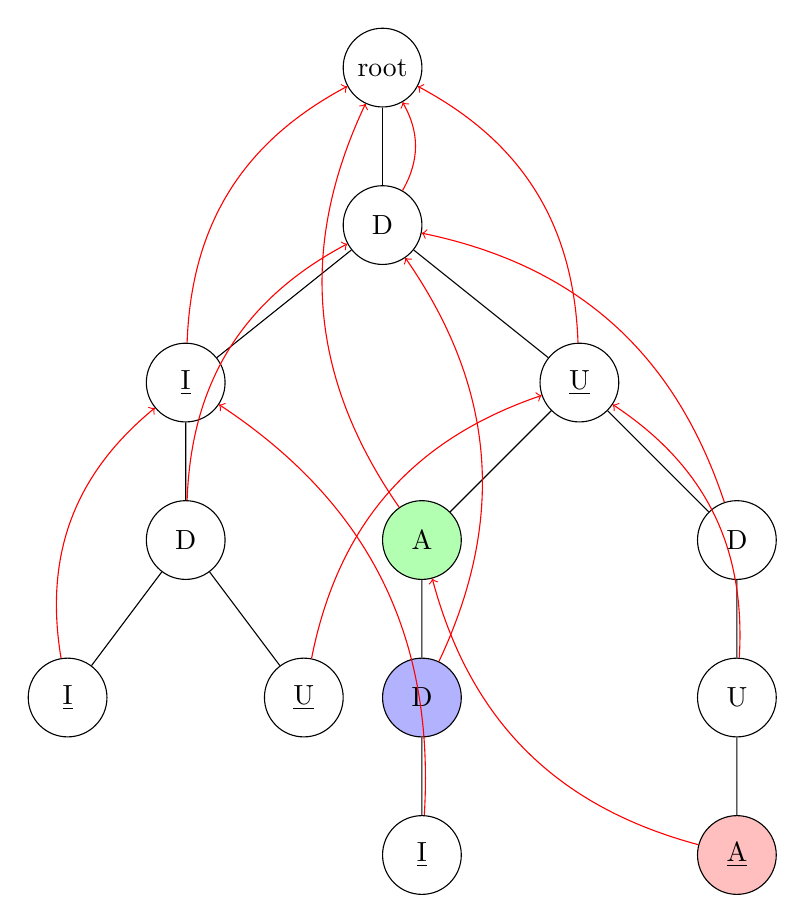
\begin{tikzpicture}[
        level 1/.style={sibling distance=6cm, level distance=2cm},
        level 2/.style={sibling distance=5cm, level distance=2cm},
        level 3/.style={sibling distance=4cm, level distance=2cm},
        level 4/.style={sibling distance=3cm, level distance=2cm},
        level 5/.style={sibling distance=2cm, level distance=2cm},
        level 6/.style={sibling distance=2cm, level distance=2ccm},
        every node/.style={circle, draw, minimum size=1cm}
    ]
        % Vẽ cây chính
        \node (root) {root}
            child { node (D1) {D}
                child { node (I) {\underline{I}}
                    child { node (D2) {D}
                        child { node (I2) {\underline{I}} }
                        child { node (U2) {\underline{U}} }
                    }
                }
                child { node (U1) {\underline{U}}
                    child { node [fill=green!30](A2) {A}
                        child { node [fill=blue!30](D4) {D}
                            child { node (I3) {\underline{I}} }
                        }
                    }
                    child { node (D3) {D}
                        child { node (U3) {U}
                            child { node [fill=pink](A) {\underline{A}} }
                        }
                    }
                }
            };

        % Thêm các liên kết về gốc
        \draw[red, ->] (D1) to[bend right] (root);
        \draw[red, ->] (I) to[bend left] (root);
        \draw[red, ->] (I2) to[bend left] (I);
        \draw[red, ->] (D2) to[bend left] (D1);
        \draw[red, ->] (U1) to[bend right] (root);
        \draw[red, ->] (D3) to[bend right] (D1);
        \draw[red, ->] (U2) to[bend left] (U1);
        \draw[red, ->] (A) to[bend left] (A2);
        \draw[red, ->] (A2) to[bend left] (root);
        \draw[red, ->] (D4) to[bend right] (D1);
        \draw[red, ->] (I3) to[bend right] (I);
        \draw[red, ->] (U3) to[bend right] (U1);
    \end{tikzpicture}

\end{center}
Number of patterns that occur in the text: 4 (DI, DIDU, DU, DUDUA).

Now text[i] = D, but node U doesn't have child node D, we trace back to the node the suffix of node U points at, which is the other node A. The other node A has child node D so we travel to that node D.
\pagebreak

\textbf{Step 10:}
\begin{center}

    \begin{table}[H]
    \centering
    \begin{tabular}{|c|c|c|c|c|c|c|c|c|c|}
    \hline
    pos   &   &   &   &   &   & i &   &   &   \\ \hline
    text  & D & I & D & U & D & U & A & D & I \\ \hline
    \end{tabular}
    \end{table}
    
    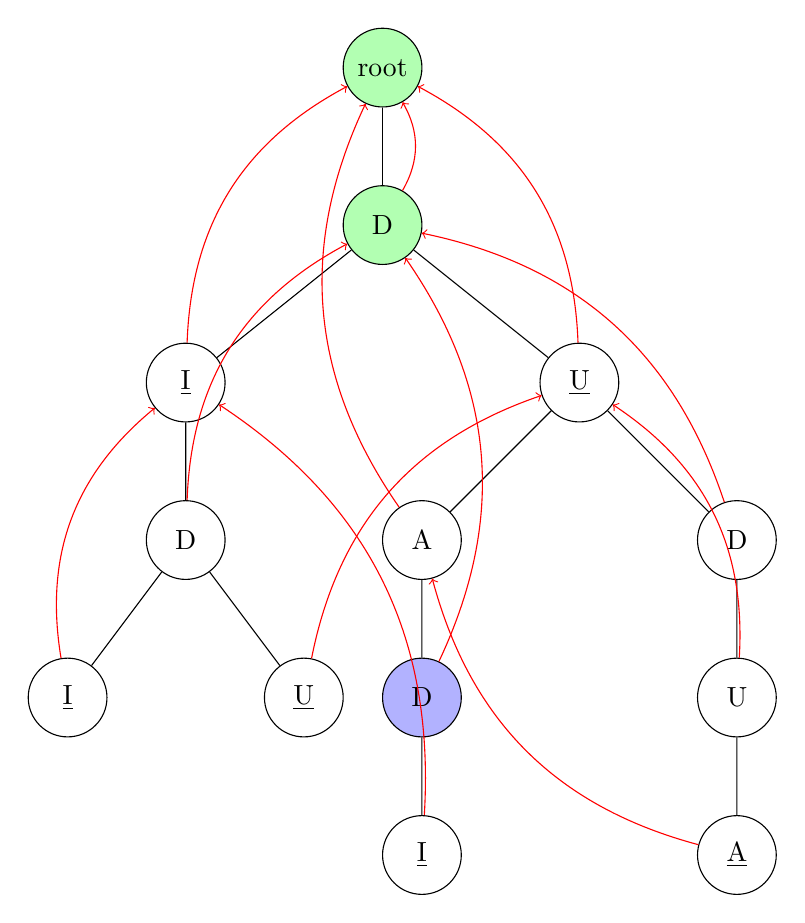
\begin{tikzpicture}[
        level 1/.style={sibling distance=6cm, level distance=2cm},
        level 2/.style={sibling distance=5cm, level distance=2cm},
        level 3/.style={sibling distance=4cm, level distance=2cm},
        level 4/.style={sibling distance=3cm, level distance=2cm},
        level 5/.style={sibling distance=2cm, level distance=2cm},
        level 6/.style={sibling distance=2cm, level distance=2ccm},
        every node/.style={circle, draw, minimum size=1cm}
    ]
        % Vẽ cây chính
        \node [fill=green!30](root) {root}
            child { node [fill=green!30](D1) {D}
                child { node (I) {\underline{I}}
                    child { node (D2) {D}
                        child { node (I2) {\underline{I}} }
                        child { node (U2) {\underline{U}} }
                    }
                }
                child { node (U1) {\underline{U}}
                    child { node (A2) {A}
                        child { node [fill=blue!30](D4) {D}
                            child { node (I3) {\underline{I}} }
                        }
                    }
                    child { node (D3) {D}
                        child { node (U3) {U}
                            child { node (A) {\underline{A}} }
                        }
                    }
                }
            };

        % Thêm các liên kết về gốc
        \draw[red, ->] (D1) to[bend right] (root);
        \draw[red, ->] (I) to[bend left] (root);
        \draw[red, ->] (I2) to[bend left] (I);
        \draw[red, ->] (D2) to[bend left] (D1);
        \draw[red, ->] (U1) to[bend right] (root);
        \draw[red, ->] (D3) to[bend right] (D1);
        \draw[red, ->] (U2) to[bend left] (U1);
        \draw[red, ->] (A) to[bend left] (A2);
        \draw[red, ->] (A2) to[bend left] (root);
        \draw[red, ->] (D4) to[bend right] (D1);
        \draw[red, ->] (I3) to[bend right] (I);
        \draw[red, ->] (U3) to[bend right] (U1);
    \end{tikzpicture}

\end{center}
Number of patterns that occur in the text: 4 (DI, DIDU, DU, DUDUA).

This node D is not the end of ant pattern so we do thing at this node. We trace back to the node the suffix of this node points at, which is the other node D. This node D is also not the end of any pattern so we do nothing at this node. We continue to trace back to the node the suffix of this node points at, which is the root. Because this is the root, we stop the procedure.
\pagebreak

\textbf{Step 11:}
\begin{center}

    \begin{table}[H]
    \centering
    \begin{tabular}{|c|c|c|c|c|c|c|c|c|c|}
    \hline
    pos   &   &   &   &   &   & i &   &   &   \\ \hline
    text  & D & I & D & U & D & U & A & D & I \\ \hline
    \end{tabular}
    \end{table}
    
    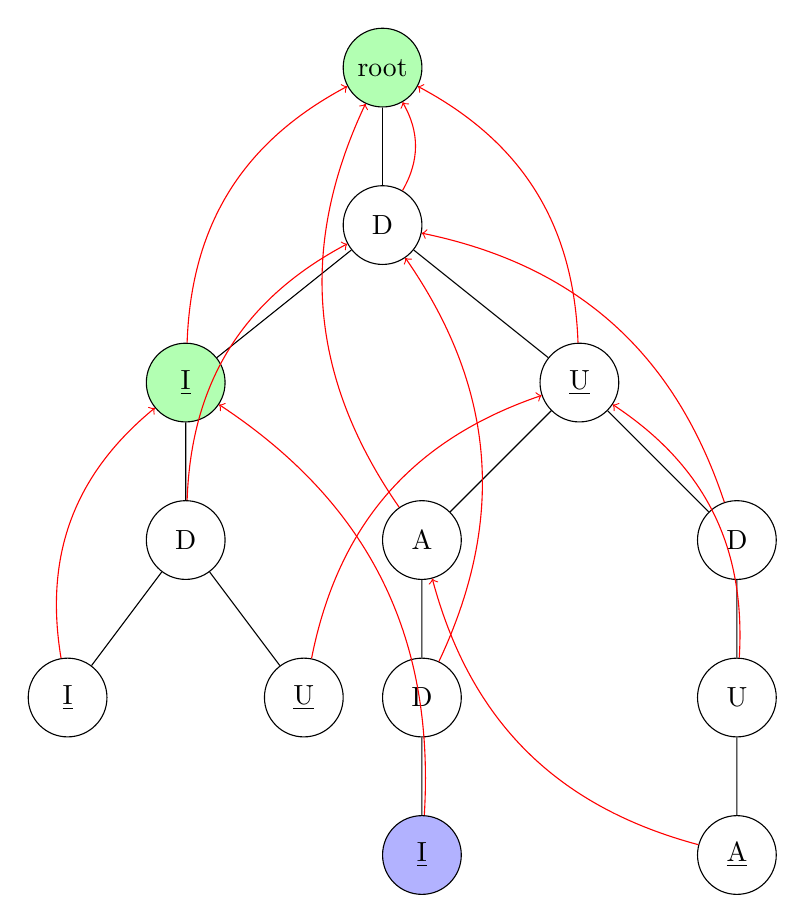
\begin{tikzpicture}[
        level 1/.style={sibling distance=6cm, level distance=2cm},
        level 2/.style={sibling distance=5cm, level distance=2cm},
        level 3/.style={sibling distance=4cm, level distance=2cm},
        level 4/.style={sibling distance=3cm, level distance=2cm},
        level 5/.style={sibling distance=2cm, level distance=2cm},
        level 6/.style={sibling distance=2cm, level distance=2ccm},
        every node/.style={circle, draw, minimum size=1cm}
    ]
        % Vẽ cây chính
        \node [fill=green!30](root) {root}
            child { node (D1) {D}
                child { node [fill=green!30](I) {\underline{I}}
                    child { node (D2) {D}
                        child { node (I2) {\underline{I}} }
                        child { node (U2) {\underline{U}} }
                    }
                }
                child { node (U1) {\underline{U}}
                    child { node (A2) {A}
                        child { node (D4) {D}
                            child { node [fill=blue!30](I3) {\underline{I}} }
                        }
                    }
                    child { node (D3) {D}
                        child { node (U3) {U}
                            child { node (A) {\underline{A}} }
                        }
                    }
                }
            };

        % Thêm các liên kết về gốc
        \draw[red, ->] (D1) to[bend right] (root);
        \draw[red, ->] (I) to[bend left] (root);
        \draw[red, ->] (I2) to[bend left] (I);
        \draw[red, ->] (D2) to[bend left] (D1);
        \draw[red, ->] (U1) to[bend right] (root);
        \draw[red, ->] (D3) to[bend right] (D1);
        \draw[red, ->] (U2) to[bend left] (U1);
        \draw[red, ->] (A) to[bend left] (A2);
        \draw[red, ->] (A2) to[bend left] (root);
        \draw[red, ->] (D4) to[bend right] (D1);
        \draw[red, ->] (I3) to[bend right] (I);
        \draw[red, ->] (U3) to[bend right] (U1);
    \end{tikzpicture}

\end{center}
Number of patterns that occur in the text: 5 (DI, DIDU, DU, DUDUA, DUADI).

Now text[i] = I, we travel to node I from node D. Because this node is the end of pattern DUADI and this pattern have not been counted, the number of patterns that occur in the text is increased by 1. We trace back to the node the suffix link of this node points at, which is other node I. This other node A is the end of pattern DI but this pattern has already been counted so we do nothing on this node. We countinue to trace back to the node the suffix of this node points at, which is the root. Because this is the root, we stop the procedure.
\subsubsection*{Result}
There are 5 patterns occur in the text DIDUDUADI.
\subsection{Complexity Analysis}
\subsubsection*{Trie Construction}
Each pattern is inserted into the trie, where the total length of all patterns is denoted as \( m \). Since inserting each character takes \( O(1) \), the total time complexity of constructing the trie is: \[ O(m) \]

\subsubsection*{Suffix Link Construction}
The suffix links are built using a depth-first search (DFS) traversal  of the trie. Each node and edge is processed once, leading to a complexity of: \[ O(m) \]

\subsubsection*{Text Searching}
Let \( n \) be the length of the text. During the search:

\begin{itemize}
    \item If a transition exists in the trie, we move forward in \( O(1) \).
    \item If there is a mismatch, suffix links guide the search backward.
\end{itemize}

\noindent In the worst case, suffix links may be followed multiple times. However, since each character in the text is processed at most once along with backtracking via suffix links, the total complexity remains: \[O(n + m)\]

\subsubsection*{Best Case}
If the text mostly follows the trie transitions without needing fail links, then each character is processed in \( O(1) \), leading to: \[ O(n) \]

\subsubsection*{Worst Case}
If suffix links are frequently used, a character may trigger multiple backtracking steps. However, across the entire search, the number of such backtracking steps is bounded by \( O(n + m) \). Thus, the worst-case complexity is: \[ O(n + m) \]

\subsubsection*{Conclusion}
The Aho-Corasick algorithm provides an efficient way to search multiple patterns in a text with the following time complexities:

\begin{itemize}
    \item \textbf{Best case:} \( O(n) \), when suffix links are rarely used.
    \item \textbf{Worst case:} \( O(n + m) \), when suffix links cause multiple jumps.
\end{itemize}